\documentclass[11pt]{article}

% Change "review" to "final" to generate the final (sometimes called camera-ready) version.
% Change to "preprint" to generate a non-anonymous version with page numbers.
\usepackage[review]{acl}

% Standard package includes
\usepackage{times}
\usepackage{latexsym}

% For proper rendering and hyphenation of words containing Latin characters (including in bib files)
\usepackage[T1]{fontenc}
% For Vietnamese characters
% \usepackage[T5]{fontenc}
% See https://www.latex-project.org/help/documentation/encguide.pdf for other character sets

% This assumes your files are encoded as UTF8
\usepackage[utf8]{inputenc}

% This is not strictly necessary, and may be commented out,
% but it will improve the layout of the manuscript,
% and will typically save some space.
\usepackage{microtype}

% This is also not strictly necessary, and may be commented out.
% However, it will improve the aesthetics of text in
% the typewriter font.
\usepackage{inconsolata}

%Including images in your LaTeX document requires adding
%additional package(s)
\usepackage{graphicx}

\usepackage{booktabs} \usepackage{multirow}

\usepackage{amsmath,amssymb}

\usepackage[ruled,vlined]{algorithm2e}
\usepackage{graphicx}
\usepackage{subcaption}
\usepackage{ulem}

\usepackage{soul}
% If the title and author information does not fit in the area allocated, uncomment the following
%
%\setlength\titlebox{<dim>}
%
% and set <dim> to something 5cm or larger.

\title{Budget-Aware Submodel Extraction from Vision-Language Foundation Models}

% Author information can be set in various styles:
% For several authors from the same institution:
% \author{Author 1 \and ... \and Author n \\
%         Address line \\ ... \\ Address line}
% if the names do not fit well on one line use
%         Author 1 \\ {\bf Author 2} \\ ... \\ {\bf Author n} \\
% For authors from different institutions:
% \author{Author 1 \\ Address line \\  ... \\ Address line
%         \And  ... \And
%         Author n \\ Address line \\ ... \\ Address line}
% To start a separate ``row'' of authors use \AND, as in
% \author{Author 1 \\ Address line \\  ... \\ Address line
%         \AND
%         Author 2 \\ Address line \\ ... \\ Address line \And
%         Author 3 \\ Address line \\ ... \\ Address line}

\author{First Author \\
  Affiliation / Address line 1 \\
  Affiliation / Address line 2 \\
  Affiliation / Address line 3 \\
  \texttt{email@domain} \\\And
  Second Author \\
  Affiliation / Address line 1 \\
  Affiliation / Address line 2 \\
  Affiliation / Address line 3 \\
  \texttt{email@domain} \\}

%\author{
%  \textbf{First Author\textsuperscript{1}},
%  \textbf{Second Author\textsuperscript{1,2}},
%  \textbf{Third T. Author\textsuperscript{1}},
%  \textbf{Fourth Author\textsuperscript{1}},
%\\
%  \textbf{Fifth Author\textsuperscript{1,2}},
%  \textbf{Sixth Author\textsuperscript{1}},
%  \textbf{Seventh Author\textsuperscript{1}},
%  \textbf{Eighth Author \textsuperscript{1,2,3,4}},
%\\
%  \textbf{Ninth Author\textsuperscript{1}},
%  \textbf{Tenth Author\textsuperscript{1}},
%  \textbf{Eleventh E. Author\textsuperscript{1,2,3,4,5}},
%  \textbf{Twelfth Author\textsuperscript{1}},
%\\
%  \textbf{Thirteenth Author\textsuperscript{3}},
%  \textbf{Fourteenth F. Author\textsuperscript{2,4}},
%  \textbf{Fifteenth Author\textsuperscript{1}},
%  \textbf{Sixteenth Author\textsuperscript{1}},
%\\
%  \textbf{Seventeenth S. Author\textsuperscript{4,5}},
%  \textbf{Eighteenth Author\textsuperscript{3,4}},
%  \textbf{Nineteenth N. Author\textsuperscript{2,5}},
%  \textbf{Twentieth Author\textsuperscript{1}}
%\\
%\\
%  \textsuperscript{1}Affiliation 1,
%  \textsuperscript{2}Affiliation 2,
%  \textsuperscript{3}Affiliation 3,
%  \textsuperscript{4}Affiliation 4,
%  \textsuperscript{5}Affiliation 5
%\\
%  \small{
%    \textbf{Correspondence:} \href{mailto:email@domain}{email@domain}
%  }
%}

\begin{document}
\maketitle

\begin{abstract}
Large vision-language foundation models (VLMs) provide strong generalization but are often over-capacitated for real-world deployment, where applications typically involve a small set of tasks and strict computational budgets. Existing approaches either incorporate budget adaptivity during pretraining or perform compression while attempting to preserve universal zero-shot capability, which inherently limits achievable compression. 
In this work, we instead formulate deployment as a \textit{task-conditioned, budget-aware submodel extraction} problem: given a pretrained model, a target task set, and a budget, the goal is to derive a structured submodel that maximizes task performance under the constraint. 
We propose a post-hoc extraction method that searches over heterogeneous structural reductions, including attention dropping, MLP dropping, block dropping, and width reduction. We rank removable units using lightweight task-aware evaluation and progressively select the operator that yields the best accuracy–budget trade-off at each reduction step. 
Without modifying the pretraining process, our approach produces task-aligned submodels that maintain strong task accuracy under tight parameter and compute budgets across multiple VLMs.
\end{abstract}


\section{Introduction}
\label{sec:intro}
The emergence of large-scale vision-language foundation models (VLMs) has fundamentally reshaped visual understanding. 
Trained on web-scale multimodal data, these models demonstrate strong generalization across diverse tasks such as 
visual question answering~\cite{antol2015vqa}, image captioning~\cite{hossain2019comprehensive,you2016image}, and multimodal reasoning~\cite{chen2024spatialvlm}. A growing number of powerful open-source VLMs are now publicly available~\cite{bai2025qwen3,liu2023visual}. Despite architectural differences, they share common characteristics: large scale, broad versatility, and strong adaptation capability. As a result, a single pretrained 
model can often serve as a universal backbone for a wide range of downstream multimodal tasks.

However, the increasing scale and universality of these models expose a mismatch with real-world deployment. Practical applications are often highly specialized and require only a narrow subset of capabilities~\cite{tan2022towards,wang2023efficientvlm,wang2025prada}. In many cases, large portions of a foundation model’s capacity become functionally redundant. For instance, an embedded vision system may only need pose estimation or anomaly detection rather than the full spectrum of dense prediction or reasoning tasks~\cite{zhuang2025argus}. Moreover, deployment environments frequently have strict computational constraints. Applications such as robotics and autonomous systems demand real-time inference under limited hardware budgets, where the parameter count and computational overhead of modern foundation models can be prohibitive. As models continue to scale for broader generalization, the gap between large-scale pretraining and budget-constrained deployment widens. Existing efforts focus primarily on improving pretraining or enhancing universal capability, yet provide limited mechanisms for deriving models that align simultaneously with specific task needs, computational budgets, and real-world deployment requirements~\cite{ma2023llm,he2024matters, zhao2025hape}.

Existing approaches to mitigate this mismatch generally fall into two categories. The first follows the once-for-all (OFA) model training~\cite{cai2019once, cai2024flextron}, where budget adaptivity is incorporated during pretraining so that sub-networks of different computational costs can be selected after training. However, such methods assume control over the pretraining process, which is often inaccessible to practitioners relying on publicly available foundation models. The second category consists of post-hoc compression techniques, including structured pruning and sparsification~\cite{he2024rethinking, he2025understanding}, which aim to reduce the size of the model while preserving overall zero-shot generalization. Because these methods seek to maintain broad universal performance, the degree of compression achievable is inherently limited. In contrast, practical deployment typically requires flexible compression levels tailored to specific budgets and focuses on a small subset of domain-specific tasks rather than universal capability~\cite{tiwari2021chipnet}. As a result, current paradigms are not explicitly designed to produce aggressively compressed submodels aligned with tasks that match the requirements of the concrete task and the budget.

In this work, we reformulate deployment as a \ul{task-conditioned, budget-constrained submodel extraction problem.} Given a pretrained VLM, a small set of target tasks, and a specified computational budget, 
our goal is to derive a structured submodel that maximizes task performance while satisfying the budget constraint. 
Instead of preserving universal zero-shot capability, we explicitly focus on aligning model capacity with the 
requirements of specific downstream tasks.
To address this problem, we propose a post-hoc extraction framework that searches over heterogeneous structural 
reductions in transformer-based vision-language models. The framework considers multiple structural operators, 
including attention removal, MLP removal, block dropping, and MLP width reduction. A lightweight task-aware ranking 
stage first estimates the relative importance of removable units, after which a granularity-controlled greedy search 
progressively selects the operator that provides the best accuracy–budget trade-off at each reduction step. 
This design enables flexible adjustment of model depth and width without modifying the original pretraining process.

By decoupling deployment adaptation from pretraining and explicitly optimizing task-specific performance, 
our approach produces task-aligned submodels that establish a clear trade-off between task accuracy and computational 
budget. This perspective provides a practical mechanism for transforming publicly available foundation models into 
budget-efficient models suitable for diverse deployment scenarios.
Our contributions are summarized as follows:

\begin{itemize}

\item \textbf{Task-Conditioned Submodel Extraction.}
We formulate deployment of vision-language foundation models as a budget-aware, task-conditioned submodel extraction problem, 
which focuses on maximizing task performance under explicit resource constraints instead of preserving universal capability.

\item \textbf{Heterogeneous Structural Extraction Framework.}
We propose a post-hoc extraction framework that searches over heterogeneous structural reductions 
(attention, MLP, block, and width) and progressively constructs submodels that achieve favorable accuracy–budget trade-offs.

\item \textbf{Comprehensive Empirical Study.}
Through systematic experiments on multiple VLM backbones, including Qwen2.5-VL and LLaVA models, 
we show that task-aligned submodel extraction consistently achieves strong accuracy under significantly reduced parameter and compute budgets.

\end{itemize}


\section{Related Work and Preliminaries}

\subsection{Once-for-all Model}

A common approach for extracting deployable submodels is Once-for-All (OFA) training~\cite{cai2019once,sakuma2023detofa}, which trains an over-parameterized supernet that supports sub-networks of different depths and widths through progressive shrinking. Related \emph{many-in-one} models~\cite{cai2024flextron,cai2025llamaflex} further introduce routing mechanisms to dynamically select submodels during inference, resembling Mixture-of-Experts (MoE) paradigms~\cite{mu2025comprehensive,zhou2022mixture}. However, these approaches require modifying the pretraining pipeline or redesigning the architecture, such as introducing routers or explicitly training a supernet. In practice, users often rely on publicly released foundation models without access to the original training process, making such approaches difficult to apply in plug-and-play deployment scenarios. In contrast, we focus on extracting efficient submodels directly from pretrained foundation models without modifying the original training procedure.

\subsection{Structure Pruning in Transformer-based Foundation Models}

Structured pruning in Transformer-based foundation models~\cite{vaswani2017attention} typically targets attention modules, MLP modules, or entire Transformer blocks. Existing methods~\cite{ma2023llm,he2024rethinking} explore different strategies, including attention drop~\cite{he2024matters}, MLP drop~\cite{mugnaini2025efficient}, block drop, and MLP width reduction~\cite{lei2025making,he2025understanding}. Attention drop mainly reduces KV-cache computation and inference latency, while MLP pruning and width reduction target the substantial redundancy in feed-forward layers. Block drop removes entire Transformer blocks but provides relatively coarse-grained control. Most prior approaches rely on a single pruning operator and aim to preserve universal or zero-shot capability across tasks. In contrast, we focus on task-conditioned submodel extraction under explicit deployment budgets, enabling more aggressive and flexible compression strategies tailored to specific downstream scenarios.

% \section{Related Work and Preliminaries}
% \subsection{Once-for-all Model}
% One important way to extract submodels from a pretrained model is to train a Once-for-All (OFA) model~\cite{cai2019once,sakuma2023detofa}. OFA training adopts a \emph{progressive shrinking} algorithm, which starts from the largest full-capacity model and gradually supports smaller submodels within a single over-parameterized supernet. The final model can flexibly instantiate sub-networks of different depths, widths, kernel sizes, or other architectural dimensions, while sharing the same set of pretrained weights across all configurations. In the context of foundation models, a closely related paradigm is often referred to as \emph{many-in-one} models~\cite{cai2024flextron,cai2025llamaflex}. These models follow a similar shrinking philosophy during training, but introduce architectural mechanisms, such as routing modules that dynamically select different submodels or computational paths at inference time. This design is conceptually related to Mixture-of-Experts (MoE) models~\cite{mu2025comprehensive,zhou2022mixture}, although the experts in these systems may have heterogeneous sizes and partially shared parameters rather than being completely independent. However, both OFA and many-in-one approaches require modifying the training pipeline or redesigning the model architecture during pretraining, for example by introducing routers, restructuring layers, or explicitly training a supernet that supports progressive shrinking. In practice, many users rely on publicly released foundation models and do not have access to the original training process, making it unrealistic to retrain models with additional architectural constraints. Consequently, while OFA-style approaches provide elegant flexibility in principle, they are difficult to apply in plug-and-play deployment scenarios where the objective is to derive efficient submodels directly from an already pretrained and fixed foundation model without modifying the original training procedure.

% \subsection{Structure Pruning in Transformer-based Foundation Models}

% Following the Transformer architecture~\cite{vaswani2017attention}, structure pruning in Transformer-based foundation models typically focuses on three structural dimensions: attention modules, MLP (feed-forward) modules, and entire Transformer blocks. Recent compression methods~\cite{ma2023llm,he2024rethinking} explore different strategies along these axes, including attention drop~\cite{he2024matters}, MLP drop~\cite{mugnaini2025efficient}, block drop, and MLP width reduction~\cite{lei2025making,he2025understanding}. Attention drop primarily aims to reduce the memory and latency overhead associated with the key-value (KV) cache during autoregressive inference, rather than significantly decreasing the total number of model parameters, since attention layers account for only a relatively small fraction of the parameters in Transformer models~\cite{he2024matters}. In contrast, MLP drop and MLP width reduction are motivated by empirical observations that MLP layers are often over-parameterized and contain substantial redundancy. As MLP modules typically dominate the parameter count in large language models, pruning or shrinking them can substantially reduce model size while maintaining competitive performance. Block drop removes entire Transformer blocks and therefore reduces both attention and MLP parameters simultaneously, but this strategy is relatively coarse-grained and often lacks fine-grained control over parameter allocation and capacity preservation. Although these pruning strategies have been widely studied individually, existing approaches typically rely on a single operator or apply pruning along a fixed structural dimension. As a result, they provide limited flexibility when adapting models to different deployment constraints. Moreover, most prior work focuses on preserving universal or zero-shot generalization across tasks. In contrast, we focus on extracting task-specific submodels under explicit resource budgets, which relaxes the requirement of maintaining universal capability and enables more aggressive compression strategies tailored to the target deployment scenario.

\begin{figure}[t]
    \centering
    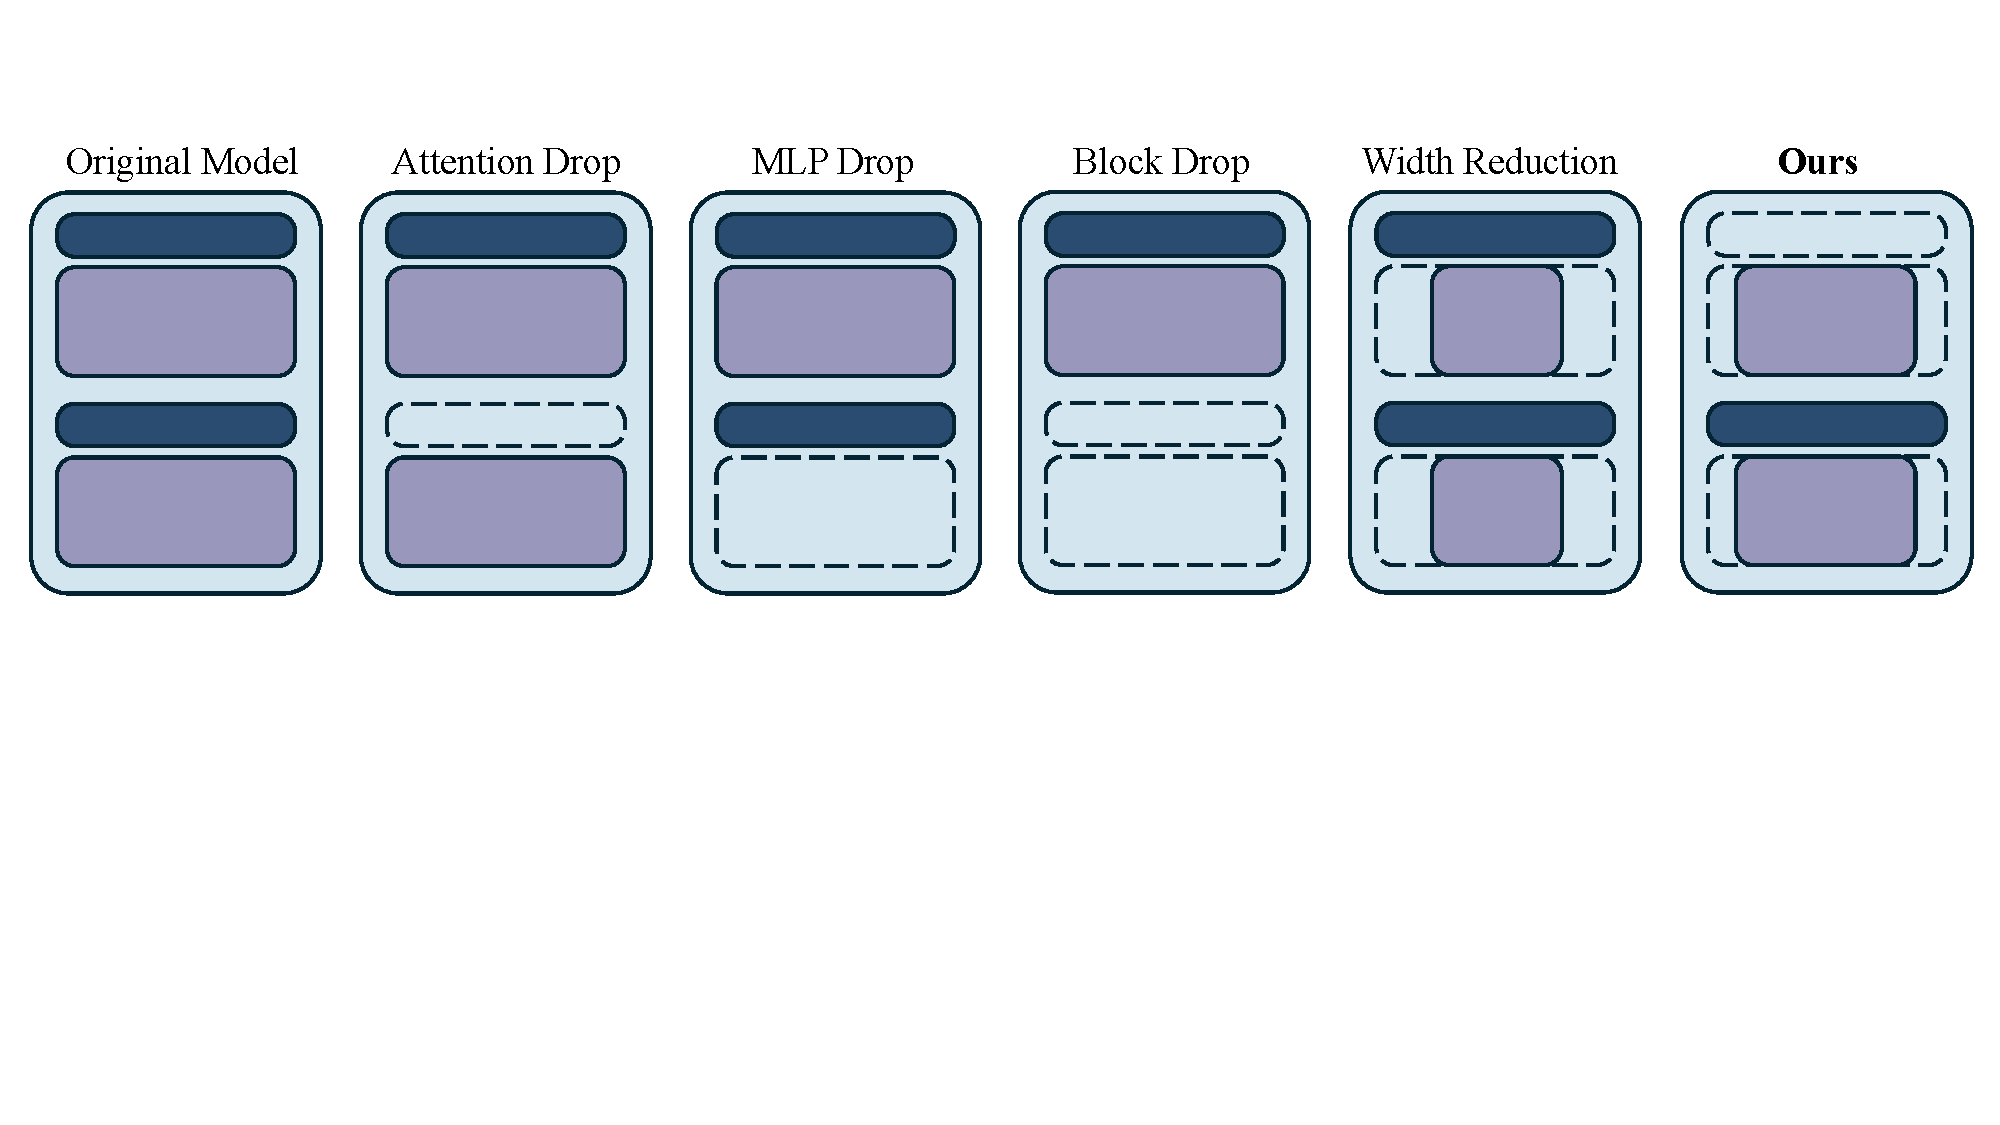
\includegraphics[width=\linewidth]{Figure/compare.pdf}
    \caption{\textbf{Structural pruning strategies in Transformer models.}
Dark blue blocks denote attention modules, purple blocks denote MLP modules,
dashed blocks indicate removed components, and narrower blocks indicate width reduction. \textbf{Ours:} We summarize the performance of different methods on VLMs and propose an automated pipeline to generate candidate sub-models by combining multiple strategies, selecting the best sub-model under target constraints.}
    \label{fig:compare}
\end{figure}

\subsection{Compression Methods in Vision-Language Models}

Since our goal is submodel extraction, we rely on structured pruning (i.e., compression) algorithms as the core tools. We therefore first conduct an empirical comparison of several representative compression strategies on common VLMs in order to understand their behavior under different deployment constraints.

For block drop, MLP drop, and MLP width reduction, we align the comparison by controlling the proportion of removed parameters relative to the total parameter count of the original model, ensuring evaluation under the same compression ratio. In contrast, attention drop removes only a small fraction of parameters and mainly improves efficiency by reducing the key-value (KV) cache during autoregressive inference; we therefore evaluate it separately. Figure~\ref{fig:compare_base} presents results on instruction fine-tuned Qwen2.5-VL-7B and LLaVA1.5-7B using VQA v2~\cite{goyal2017making} and MMBench~\cite{liu2024mmbench}. Empirically, under the same parameter drop ratio, MLP width reduction generally preserves performance better than block drop and MLP drop, particularly at higher compression levels. This observation suggests that, in our evaluated settings, redundancy in these VLMs is more concentrated in the width of MLP layers rather than in model depth. We also observe that, under comparable compression ratios and benchmarks, Qwen2.5-VL-7B tends to exhibit steeper performance degradation than LLaVA1.5-7B, indicating relatively lower redundancy in the former model within our experimental setup.


\begin{figure*}[t]
    \centering

    \begin{subfigure}[t]{0.49\linewidth}
        \centering
        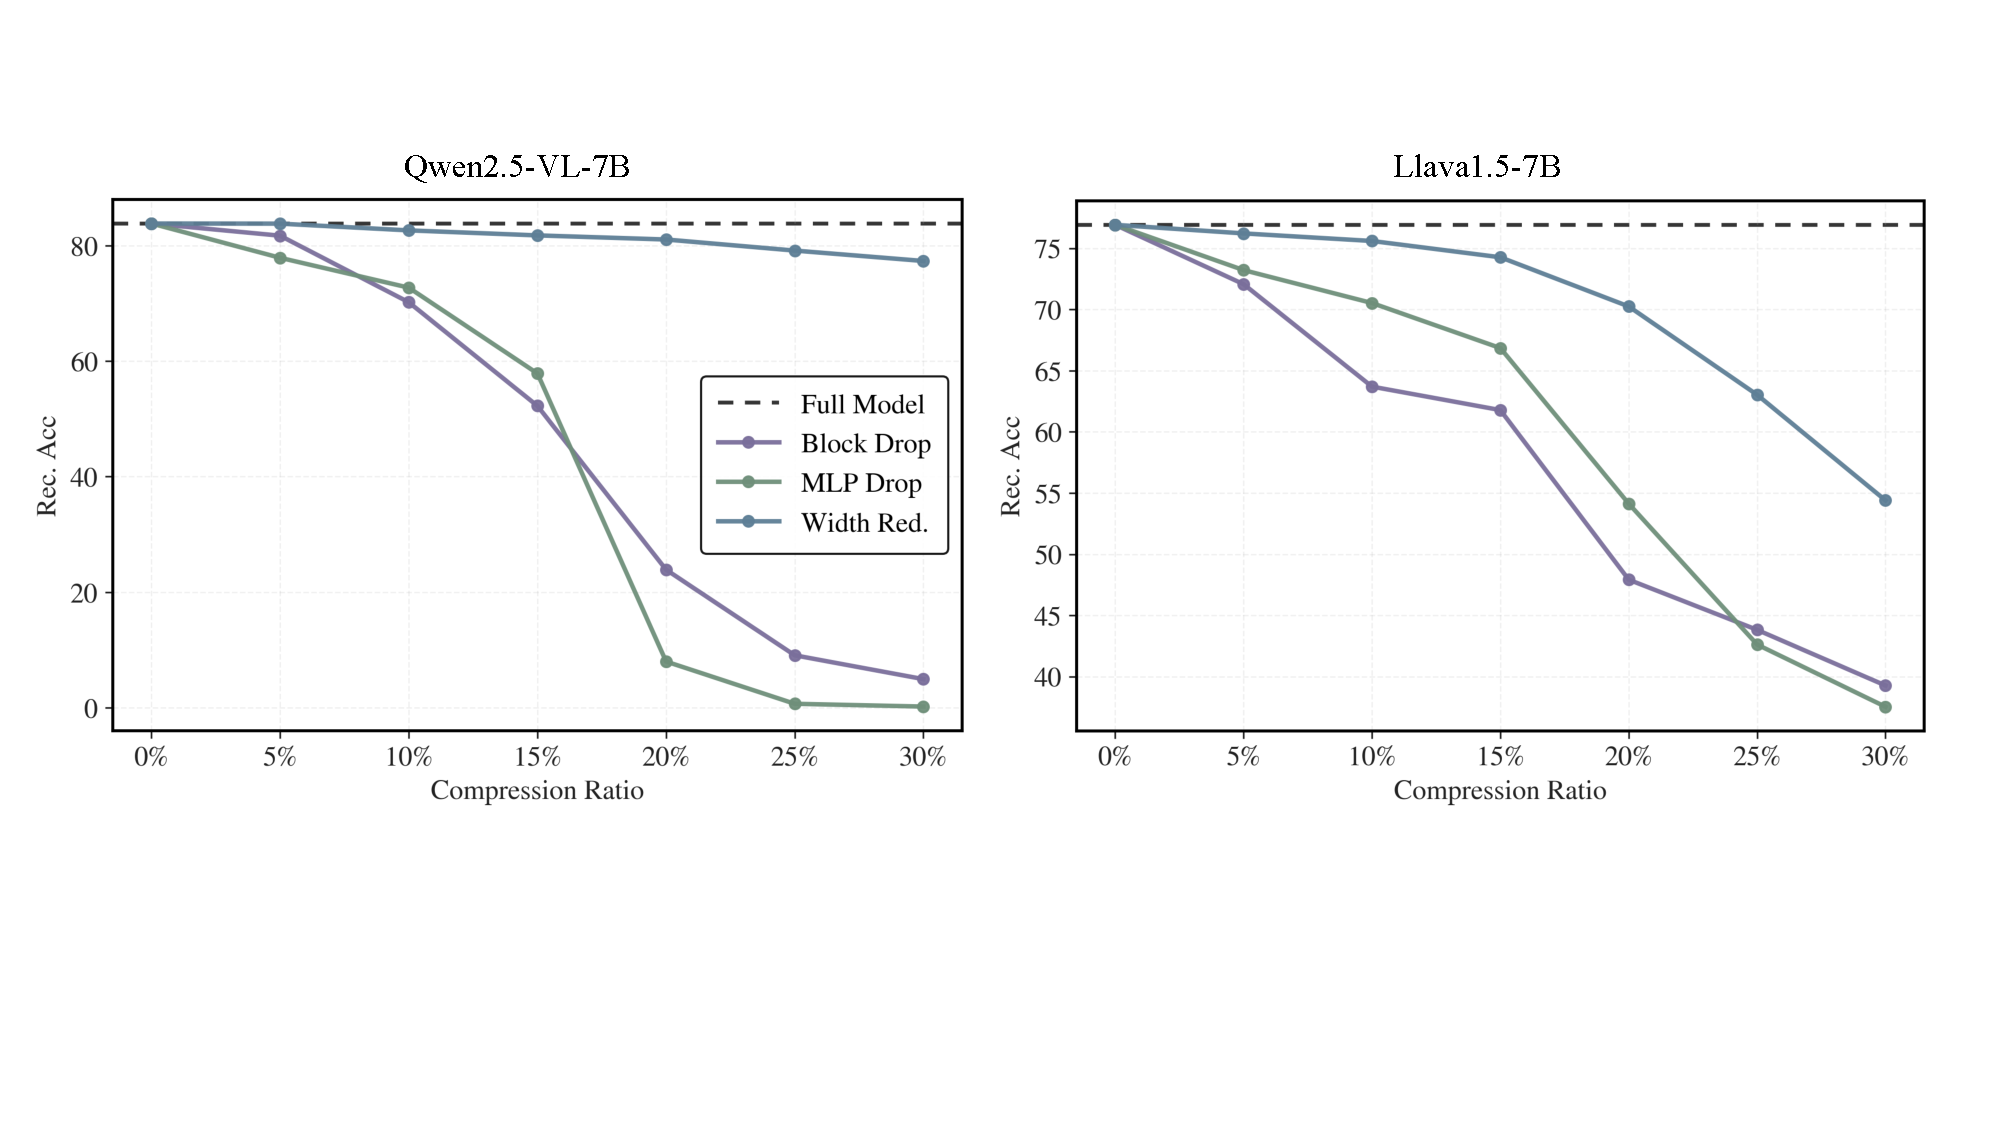
\includegraphics[width=\linewidth]{Figure/qwen_baseline.pdf}
        \caption{Performance of different compression methods on VQA v2.}
        \label{fig:compare_base}
    \end{subfigure}
    \hfill
    \begin{subfigure}[t]{0.49\linewidth}
        \centering
        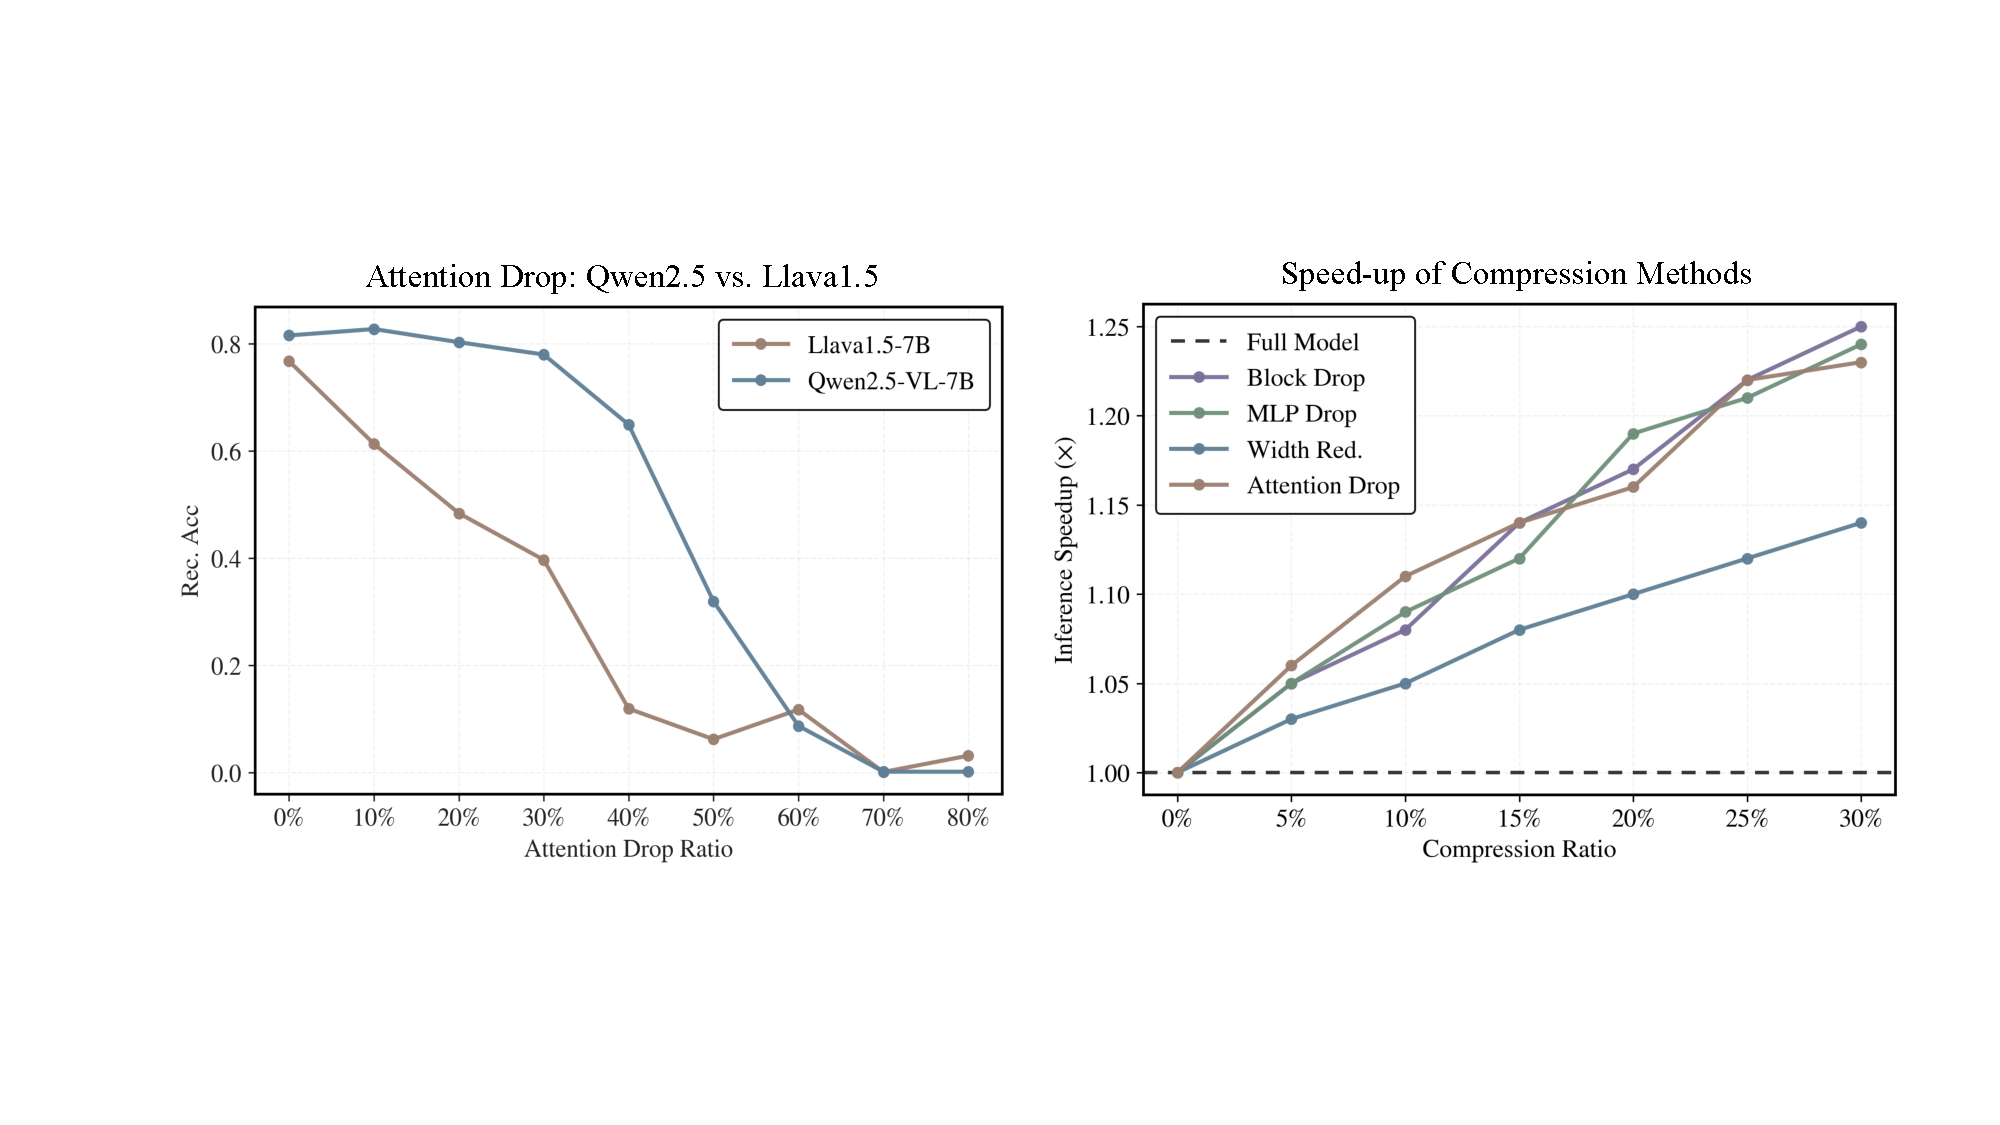
\includegraphics[width=\linewidth]{Figure/attention.pdf}
        \caption{Attention drop performance and inference speedup.}
        \label{fig:atten_com}
    \end{subfigure}

    \caption{Comparison of different compression methods on Qwen2.5-VL and LLaVA1.5 7B models.}
    \label{fig:combined}
\end{figure*}

% \begin{figure*}[t]
%     \centering
%     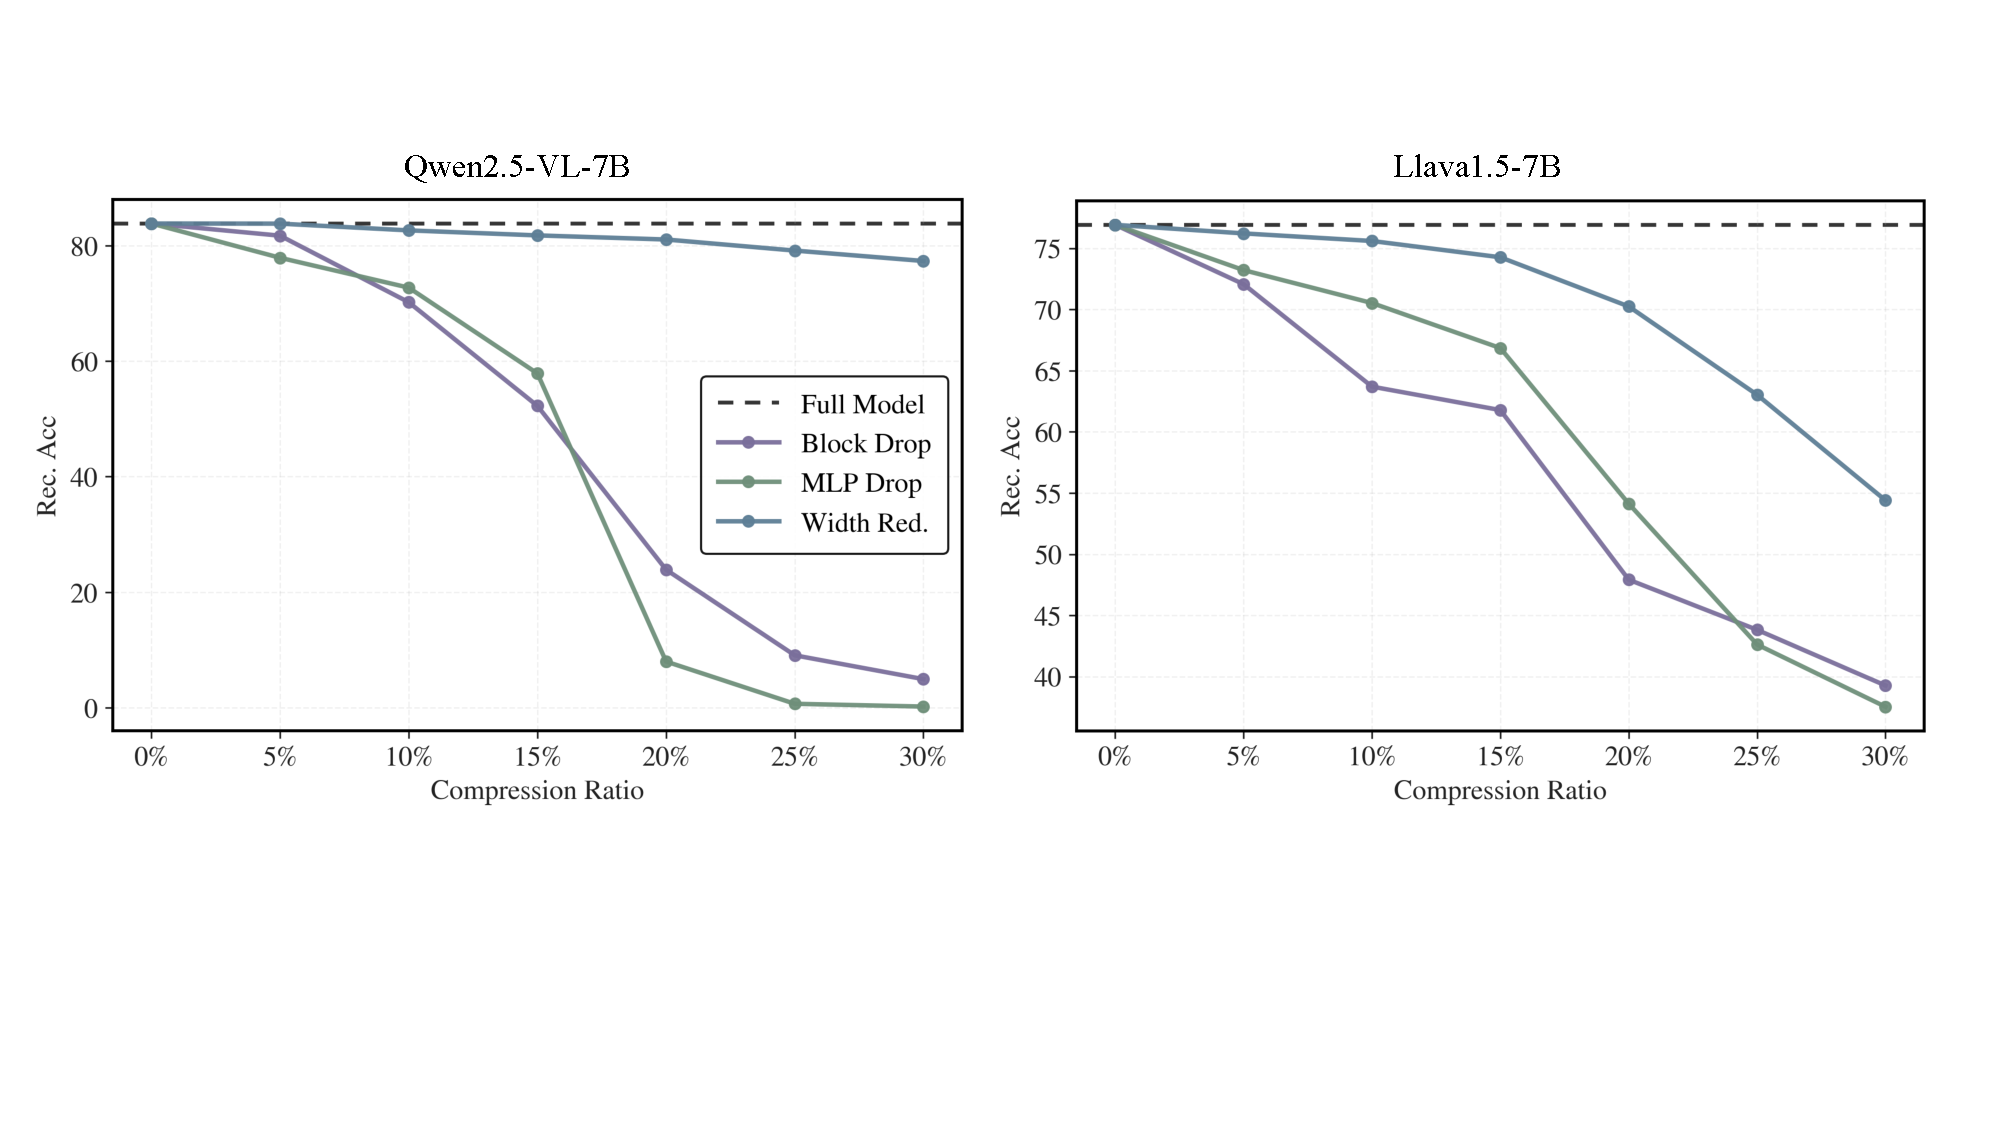
\includegraphics[width=\linewidth]{Figure/qwen_baseline.pdf}
%     \caption{The performance of different compression methods in 7B Qwen2.5-VL and Llava1.5 models. The performance is evaluated on VQA v2. Different compression methods share the same ratio of dropped parameters to the total number of parameters.}
%     \label{fig:compare_base}
% \end{figure*}

For attention drop, which is more effective for reducing GPU memory usage and inference latency than for reducing parameter count~\cite{he2024matters,heuncovering}, we conduct additional experiments to analyze its efficiency characteristics. As shown in Figure~\ref{fig:atten_com}, dropping less than 30\% of attention layers in Qwen and LLaVA models largely preserves VLM performance. Although this operation removes less than 3\% of the total model parameters, it provides noticeable inference speed improvements due to the reduction of KV-cache computation during autoregressive decoding. This efficiency gain is comparable to that achieved by substantially larger parameter reductions through width reduction. These observations indicate that different compression operators affect model efficiency and parameter count in different ways. Therefore, extracting an optimal submodel requires considering the primary deployment bottleneck, such as parameter-constrained scenarios (favoring MLP reduction) or latency-constrained scenarios (favoring attention drop).


% \begin{figure*}[t]
%     \centering
%     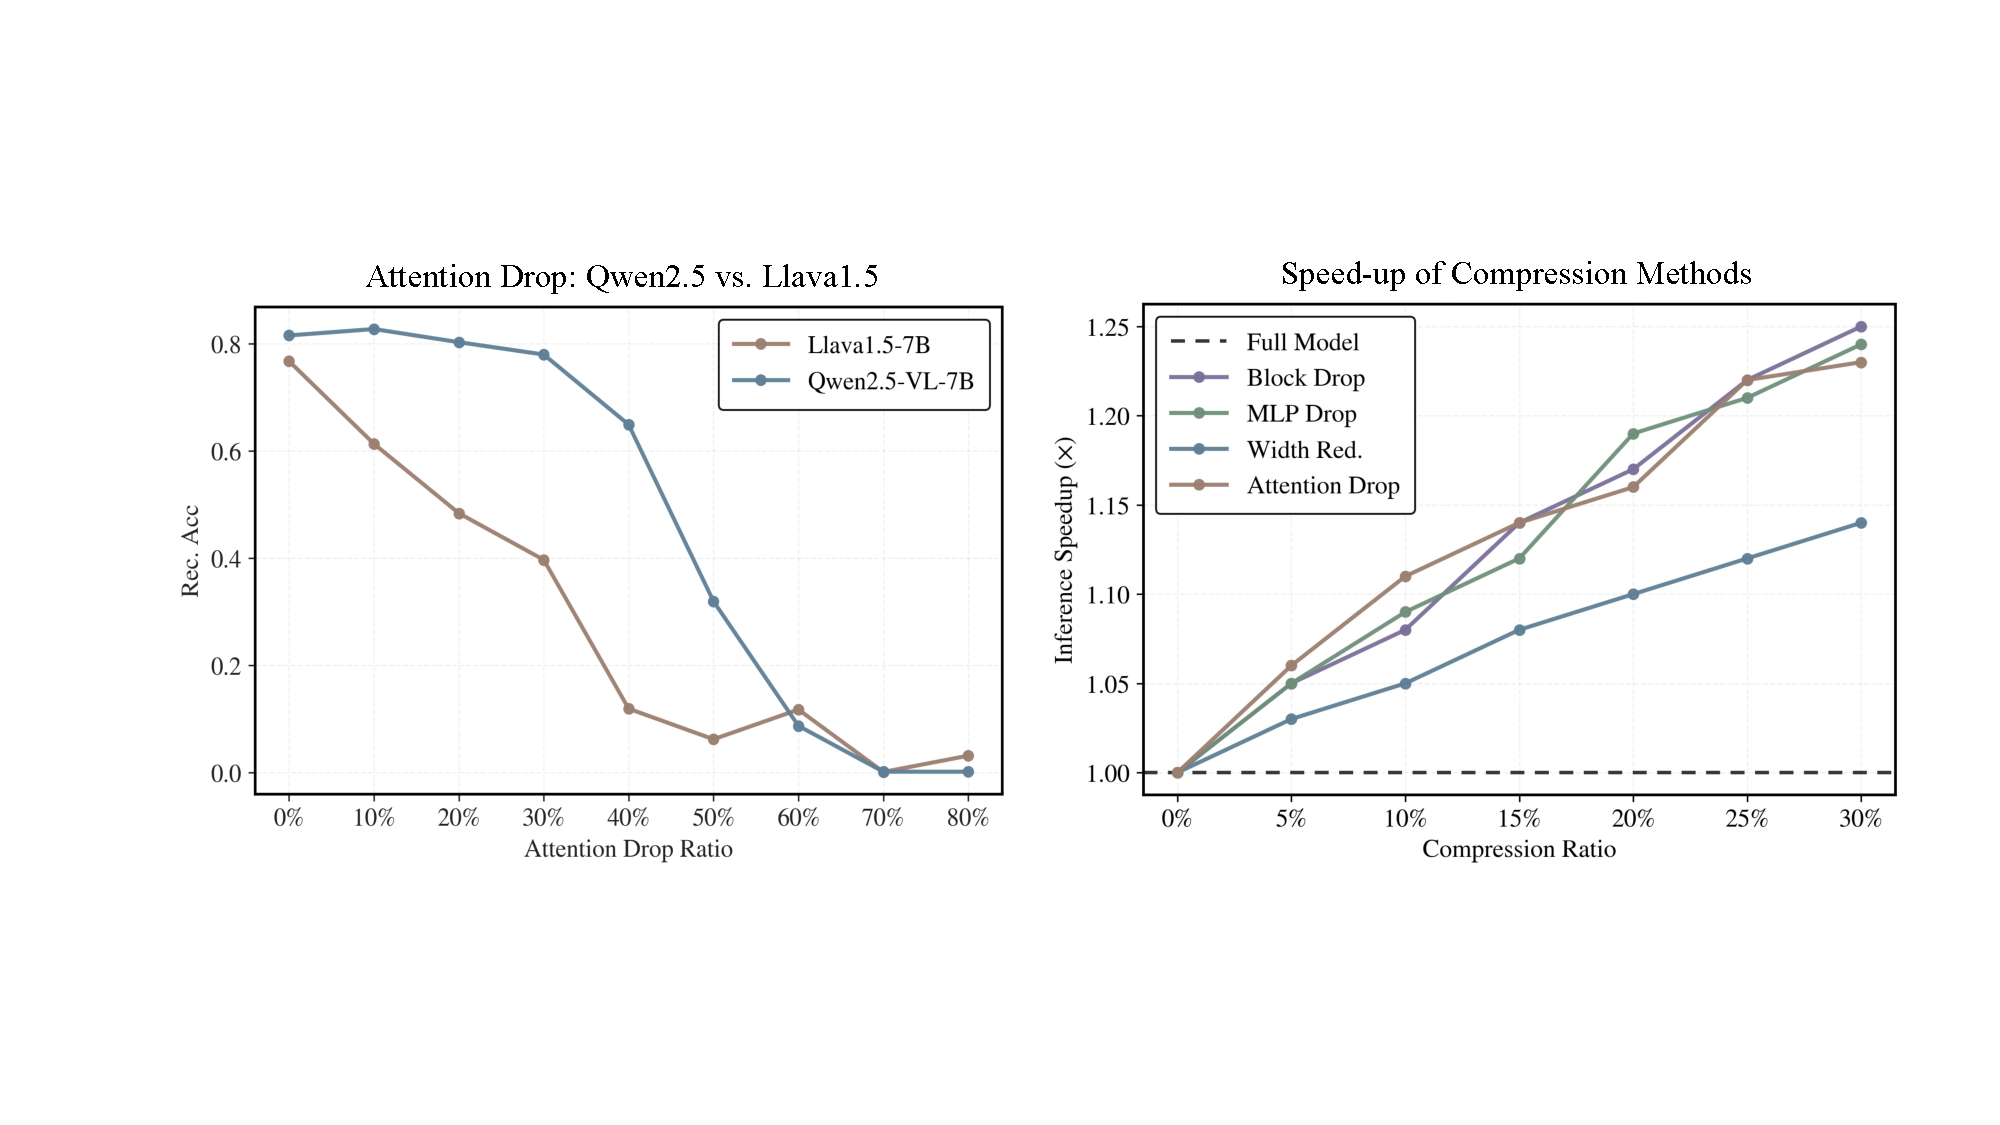
\includegraphics[width=\linewidth]{Figure/attention.pdf}
%     \caption{The performance of attention drop in 7B Qwen2.5-VL and Llava1.5 models and the inference speedup compared to mlp-related compression methods.}
%     \label{fig:atten_com}
% \end{figure*}


\section{Method}

\subsection{Problem Setup}

Let $F(\theta)$ denote a pretrained VLM, where $\theta$ represents the full set of model parameters. We denote the original parameter size by $P_{\mathrm{orig}} = |\theta|$. We consider a small set of downstream tasks $\mathcal{T} = \{T_1, \dots, T_k\}$, where typically $k \in [1,3]$. These tasks represent the target deployment scenario and correspond to a small number of task-specific benchmarks. We evaluate performance using the averaged validation accuracy across the selected tasks, denoted as $\mathrm{Acc}(F(\theta))$.

Given a target parameter budget $B \le P_{\mathrm{orig}}$, our goal is to extract a structured submodel $F(\theta')$ with parameter size $P' = |\theta'| \le B$, such that its performance on the target tasks is maximized.

Formally, we aim to solve:
\begin{equation}
\max_{\theta' \subseteq \theta} \ \mathrm{Acc}\big(F(\theta')\big)
\quad
\text{s.t.}
\quad
|\theta'| \le B.
\end{equation}

We emphasize that the objective is explicitly task-conditioned: instead of preserving universal zero-shot capability, we seek the best-performing submodel under a specified parameter constraint for the selected target tasks.

\subsection{Model-Level Ranking under the Original Model}

Before performing budgeted reduction, we first compute an importance ranking for removable structural units based on the original pretrained model. This ranking stage provides a coarse estimate of the relative importance of different components and serves as a candidate ordering for the subsequent extraction process.

For block-level ranking, suppose the model contains $L$ Transformer blocks. We construct $L$ temporary variants, each removing exactly one block while keeping all other components unchanged. Each variant is evaluated on a lightweight validation subset consisting of $K$ batches ($KB$ samples in total). Blocks whose removal yields higher accuracy are considered less important, and blocks are ranked accordingly. The same procedure is applied to attention modules and MLP sub-layers: each unit is individually removed once, and its post-removal accuracy determines its ranking.

For MLP channels, instead of repeatedly measuring validation accuracy, we estimate importance using output sensitivity. Given intermediate activation $h$ and output projection weight $W_d$, the contribution of channel $i$ is approximated by the magnitude of $W_{d,i} h_i$. Each MLP layer is ranked independently based on this criterion.
After this stage, we obtain a ranking over blocks, attention modules, MLP modules, and channels. Because the evaluation subset is extremely lightweight, this ranking step can be computed efficiently and performed only once before the extraction process. For attention layers, we follow the selection method in \cite{he2024matters}.

% \begin{algorithm}[t]
% \caption{Granularity-Controlled Submodel Extraction}
% \label{alg:greedy_extract_rank}
% \KwIn{Pretrained model $F(\theta)$; target budget $B$; reduction unit $g$ (size of one MLP); lightweight set $\mathcal{D}_{\text{lite}}$ ($K$ batches, $KB$ samples)}
% \KwOut{Structured submodel parameters $\theta'$ with $|\theta'|\le B$}

% \textbf{Stage 1: Ranking on the original model.}\;

% For each removable structural unit $u$, compute its drop score on $\mathcal{D}_{\text{lite}}$:
% $s(u)=\mathrm{Acc}(F(\theta_{-u});\mathcal{D}_{\text{lite}})$.

% For each MLP layer $\ell$ and channel $i$, compute a channel importance score:
% $s_{\ell,i}=\mathbb{E}_{x\sim\mathcal{D}_{\text{lite}}}\!\left[|W^{(\ell)}_{d,i}h^{(\ell)}_i|\right]$.

% Initialize $\theta^{(0)} \leftarrow \theta$ and $t \leftarrow 0$.

% \textbf{Stage 2: Budget-aware extraction with fixed granularity.}\;
% \While{$|\theta^{(t)}| - g > B$}{
%     \tcp{Candidate set = next available units whose size is approximately $g$}
%     $\mathcal{C}^{(t)} \leftarrow \emptyset$\;
%     Add the next not-yet-dropped unit from each ranking (block, attention, or MLP) into $\mathcal{C}^{(t)}$\;

%     \ForEach{$a \in \mathcal{C}^{(t)}$}{
%         Apply $a$ to obtain a temporary submodel $F(\theta^{(t)}_{a})$\;
%         Evaluate $A(a)=\mathrm{Acc}\big(F(\theta^{(t)}_{a});\mathcal{D}_{\text{lite}}\big)$\;
%     }
%     $a^{(t)} \leftarrow \arg\max_{a\in\mathcal{C}^{(t)}} A(a)$\;
%     $\theta^{(t+1)} \leftarrow \theta^{(t)}_{a^{(t)}}$\;
%     Advance the iterator only for the ranking type selected by $a^{(t)}$\;
%     $t \leftarrow t+1$\;
% }

% \textbf{Stage 3: Final budget matching by width reduction.}\;
% Let remaining reduction be $\Delta = |\theta^{(t)}| - B$.\;
% Shrink MLP widths to remove approximately $\Delta$ parameters.\;
% Return the final submodel parameters $\theta'$.
% \end{algorithm}

% \begin{algorithm}[htbp]
% \caption{Granularity-Controlled Submodel Extraction}
% \label{alg:greedy_extract_rank}
% \KwIn{Pretrained model $F(\theta)$; target budget $B$; reduction unit $g$ (size of one MLP);
% lightweight set $\mathcal{D}_{\text{lite}}$ ($K$ batches, $KB$ samples)}
% \KwOut{Structured submodel parameters $\theta'$ with $|\theta'|\le B$}

% \textbf{Stage 1: Ranking on the original model.}\;

% For each removable structural unit $u$,
% compute its drop score on $\mathcal{D}_{\text{lite}}$:
% \[
% s(u) = \mathrm{Acc}(F(\theta_{-u}); \mathcal{D}_{\text{lite}}).
% \]

% For each MLP layer $\ell$ and channel $i$,
% compute a channel importance score:
% \[
% s_{\ell,i} = \mathbb{E}_{x\sim\mathcal{D}_{\text{lite}}}
% \big[\, | W^{(\ell)}_{d,i} h^{(\ell)}_i | \,\big].
% \]

% Initialize $\theta^{(0)} \leftarrow \theta$ and $t \leftarrow 0$.

% \BlankLine
% \textbf{Stage 2: Budget-aware extraction with fixed granularity.}\;
% \While{$|\theta^{(t)}| - g > B$}{
%     \tcp{Candidate set = next available units whose size is approximately $g$}
%     $\mathcal{C}^{(t)} \leftarrow \emptyset$\;
%     Add the next not-yet-dropped unit from each ranking (block, attention, or MLP) into $\mathcal{C}^{(t)}$\;

%     \ForEach{$a \in \mathcal{C}^{(t)}$}{
%         Apply $a$ to obtain a temporary submodel $F(\theta^{(t)}_{a})$\;
%         Evaluate $A(a)=\mathrm{Acc}\big(F(\theta^{(t)}_{a}); \mathcal{D}_{\text{lite}}\big)$\;
%     }
%     $a^{(t)} \leftarrow \arg\max_{a\in\mathcal{C}^{(t)}} A(a)$\;
%     $\theta^{(t+1)} \leftarrow \theta^{(t)}_{a^{(t)}}$\;
%     Advance the iterator only for the ranking type selected by $a^{(t)}$\;
%     $t \leftarrow t+1$\;
% }

% \BlankLine
% \textbf{Stage 3: Final budget matching by width reduction.}\;
% Let remaining reduction be $\Delta = |\theta^{(t)}| - B$\;
% Shrink MLP widths to remove approximately $\Delta$ parameters by pruning the lowest-ranked channels per layer\;
% Return the final submodel parameters $\theta'$.
% \end{algorithm}

\subsection{Granularity-Controlled Submodel Extraction}

Based on the precomputed ranking, we perform budget-aware submodel extraction in a step-wise manner. Empirically, removing an entire MLP sub-layer provides a stable and effective reduction unit in transformer-based VLMs. We therefore adopt the parameter size of one MLP as the default reduction granularity, which allows the extraction process to proceed with consistent parameter reductions at each step. This design effectively performs operator-level search
over heterogeneous structural reductions under a fixed
budget constraint.

For example, if the target requires removing approximately 50\% of parameters and one MLP corresponds to about 5\% of the total parameters, we perform roughly 10 reduction steps. At each step, we consider candidate structural reductions across different operator types (block removal, attention removal, or MLP removal) that correspond to approximately one reduction unit. Each candidate submodel is evaluated on the lightweight validation subset, and the operator that achieves the highest validation accuracy is selected. This step-wise selection process progressively constructs the final submodel while respecting the parameter budget.
The procedure continues until the cumulative parameter reduction slightly exceeds the target budget. Finally, we apply MLP width reduction to finely adjust the remaining parameter count and match the target constraint precisely. The same extraction framework can also be applied under
an inference speed budget by selecting operators that
reduce computational latency.

This design tightly couples the ranking stage with the extraction process: the ranking restricts the candidate pool of removable components, while the granularity-controlled selection determines the combination of structural operators used in the final hybrid submodel.


\section{Experiments}

\subsection{Experimental Setup}

\textbf{Models and Submodel Settings.}
We evaluate our method on four widely used instruction-following VLM backbones:
Qwen2.5-VL-7B, Qwen2.5-VL-3B~\cite{xu2025qwen25vltechnicalreport}, LLaVA-1.5-7B, and LLaVA-1.5-13B~\cite{liu2023visual}.
Unless otherwise specified, we keep the vision encoder frozen during extraction and recovery training, and apply all structural modifications to the language-side Transformer.

\textbf{Benchmarks and Datasets.}
We use three VQA-style benchmarks as target tasks: VQA v2~\cite{goyal2017making}, MMBench~\cite{liu2024mmbench}, and TextVQA~\cite{singh2019towards}, and report accuracy as the evaluation metric.
For each benchmark, we sample 2,000 validation/test examples for evaluation to keep experiments consistent and computationally tractable.
For the lightweight ranking stage, we use a much smaller fixed subset of 64 samples, which is shared across all candidate evaluations.

\textbf{Recovery Training Details.}
After submodel extraction, we optionally perform lightweight recovery training for 1 epoch on 5,000 training samples with learning rate $1\times10^{-6}$ using bf16 mixed precision.
We sweep target compression ratios over $\{5\%, 10\%, 15\%, 20\%, 25\%, 30\%\}$ parameter reduction and $\{5\%, 10\%, 15\%, 20\%, 25\%, 30\%\}$ inference speedup.
Throughout the experiments, we use the parameter size of one MLP layer as the default reduction unit to define the step granularity in our extraction procedure, and one attention layer as the default inference speedup unit. All experiments are conducted on NVIDIA H200 GPUs. Peak memory occupation is calculated on one GPU. We use AI tools to help developing the evaluation code.

\begin{figure*}[t]
    \centering
    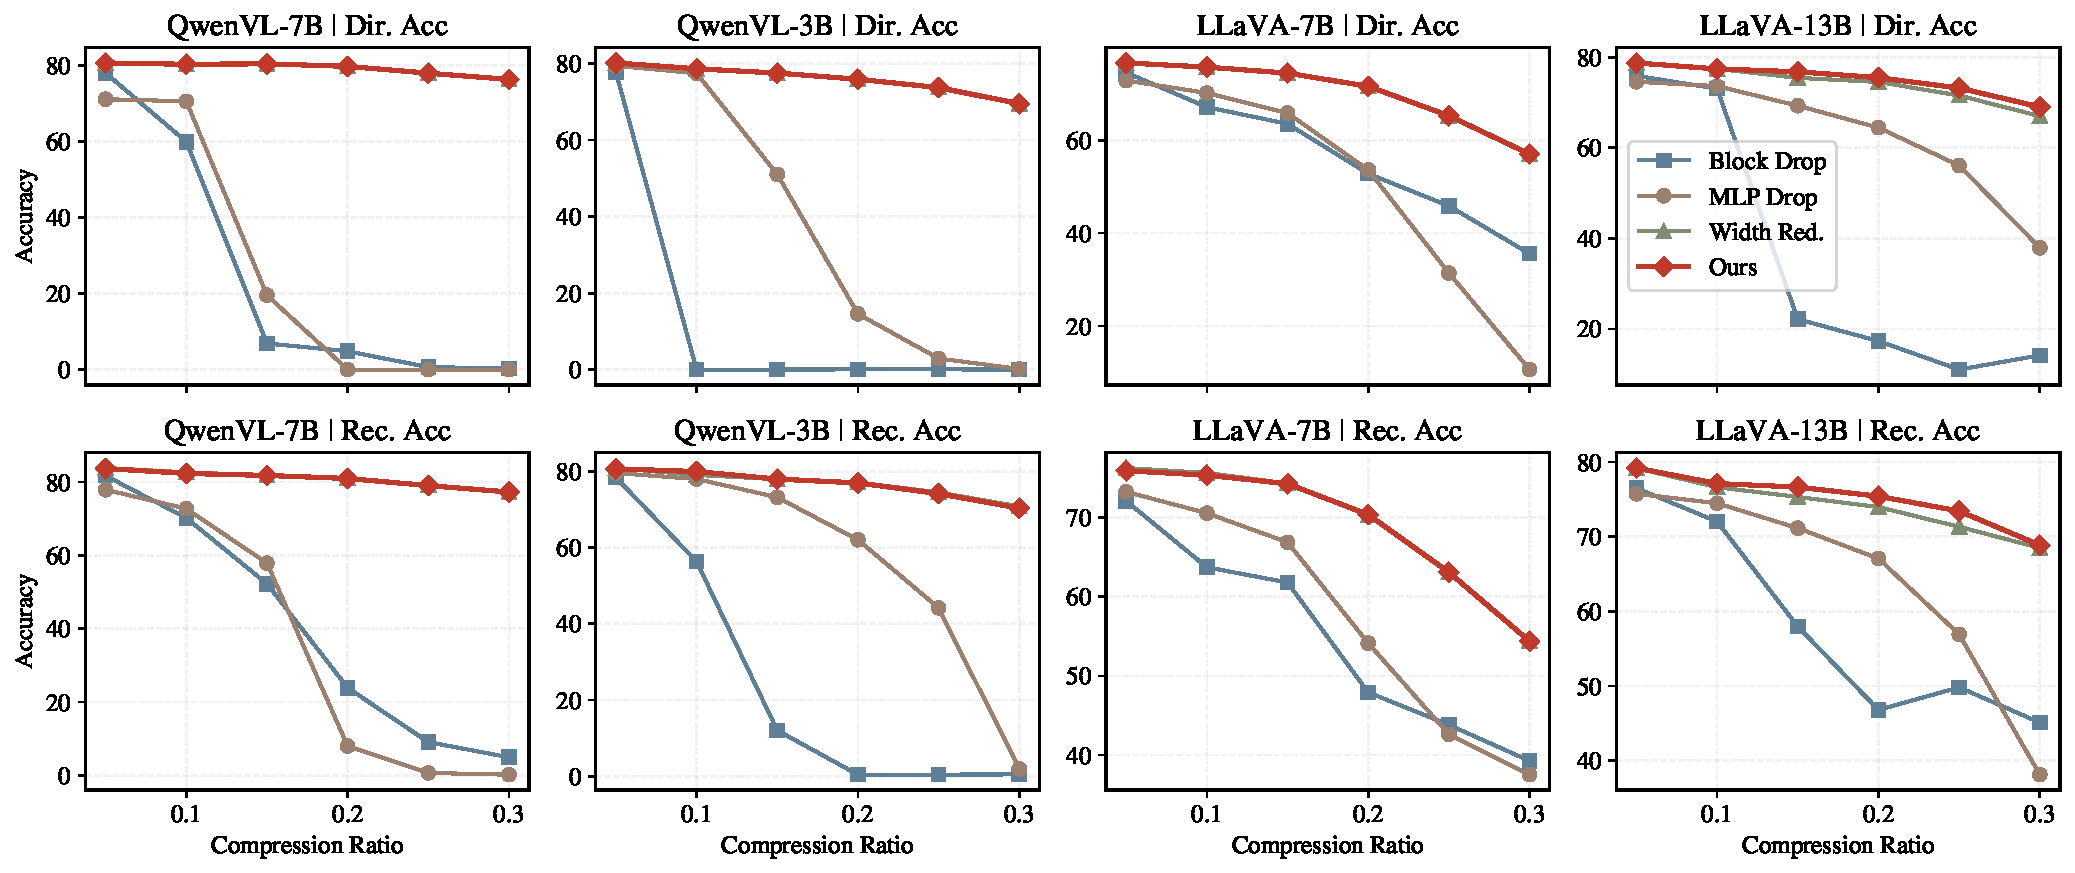
\includegraphics[width=\linewidth]{Figure/compression_parameter.pdf}
    \caption{\textbf{Submodel performance under parameter-budgeted compression. Attention drop is excluded since it removes very few parameters.}
    We compare different drop operators across four models. For each model, the top row reports the direct accuracy of the compressed submodel (Dir. Acc) and the bottom row reports the recovered accuracy after recovery training (Rec. Acc). We exclude attention drop since it is consistently inferior under parameter-budgeted settings.
    Overall, width reduction yields the strongest accuracy retention across compression ratios, and our method adapts to select the most suitable operator to match the budget while maintaining accuracy competitive with the best baseline.}
    \label{fig:param_budget_8plots}
\end{figure*}

\begin{figure*}[t]
    \centering
    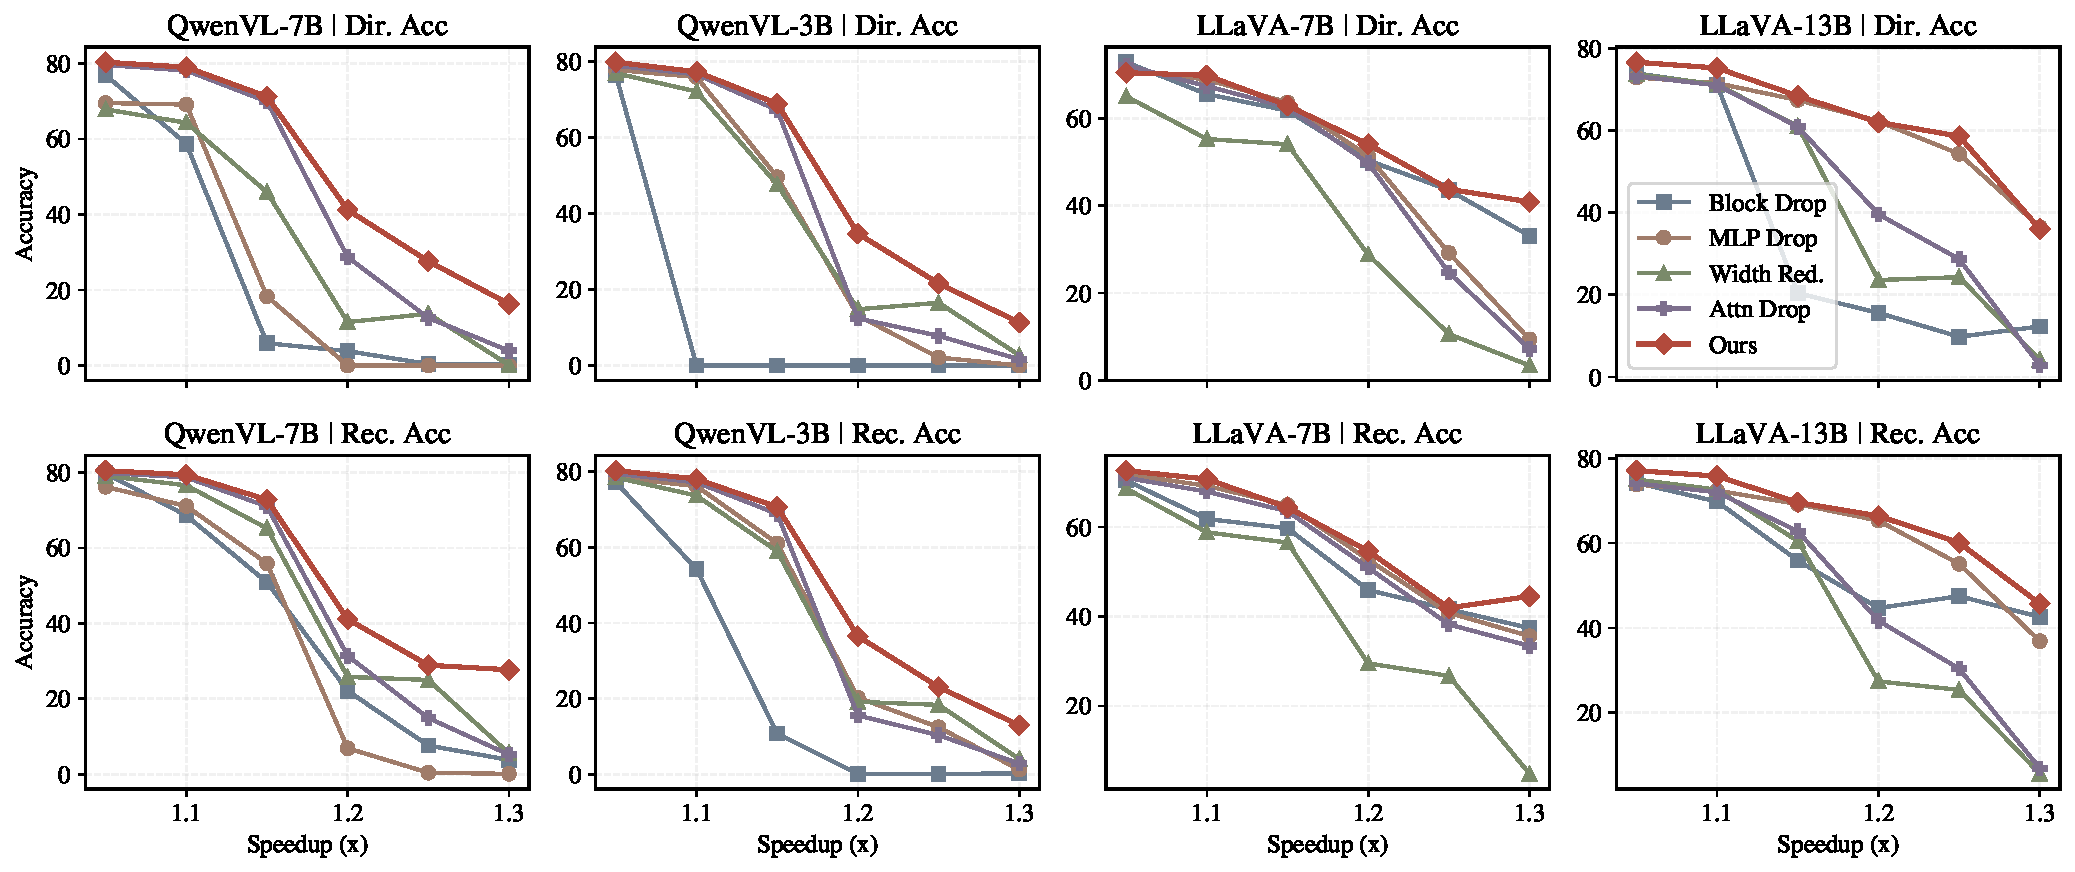
\includegraphics[width=\linewidth]{Figure/compression_inf.pdf}
\caption{Submodel extraction under an inference speed budget. 
Our method adaptively selects among heterogeneous operators and achieves consistently strong performance across different speed-up targets.}
    \label{fig:inf_budget_8plots}
\end{figure*}

\subsection{Submodel Extraction Performance}

We first study submodel extraction when the deployment constraint is defined by the \textbf{parameter budget}. 
Figure~\ref{fig:param_budget_8plots} summarizes the accuracy trends across four backbones and multiple compression ratios. 
A consistent observation is that \textbf{MLP width reduction is the most accuracy-preserving operator under parameter-budgeted compression}. 
Compared to dropping entire blocks or MLP modules, width reduction removes parameters in a finer-grained manner while preserving the overall network structure, which helps maintain the representational capacity required for VQA tasks. 
This pattern holds consistently across all evaluated models and for both direct accuracy and recovered accuracy.

Although width reduction performs strongly under parameter constraints, it is not always the optimal choice at every operating point. 
Our framework is designed to \textbf{adaptively select the operator that best matches the current budget–accuracy trade-off}. 
As shown in Figure~\ref{fig:param_budget_8plots}, the extracted submodels consistently achieve performance comparable to or better than the strongest single-operator baseline across most compression ratios. 
This behavior indicates that combining heterogeneous operators can exploit complementary effects: width reduction is chosen when it provides the best parameter–accuracy trade-off, while other operators are selected when they produce better local improvements.

We next analyze submodel extraction when the deployment constraint is defined by the \textbf{inference speed budget}. 
Figure~\ref{fig:inf_budget_8plots} presents the accuracy trends under different speed-up targets. 
In contrast to the parameter-budget scenario, width reduction is no longer consistently the most favorable operator. 
When the required speed-up is relatively small, \textbf{attention drop} typically achieves the highest accuracy, since removing attention layers directly reduces the key-value cache computation during autoregressive decoding while affecting only a small portion of the model parameters.
As the required speed-up increases, \textbf{block drop} becomes more effective. 
Removing entire Transformer blocks shortens the computational path of the network and therefore provides stronger latency reduction than attention removal alone. 
In comparison, width reduction offers relatively limited latency benefits despite reducing parameters, because shrinking intermediate tensor dimensions does not always translate to proportional improvements in GPU kernel efficiency.

Overall, these results highlight the importance of \textbf{adaptive operator selection under different deployment constraints}. 
While width reduction dominates under parameter budgets, latency-oriented deployment favors operators that directly reduce computation, such as attention removal and block removal. 
Our extraction framework can automatically adapt to these different optimization objectives and consistently produce high-performing submodels across both parameter- and latency-budget settings.


\begin{table}[t]
\centering

\resizebox{\linewidth}{!}{
\begin{tabular}{cc|ccc}
\toprule
\multicolumn{2}{c}{\textbf{Method}} 
& \multirow{2}{*}{\shortstack{\textbf{Peak}\\\textbf{Alloc.(GB) $\downarrow$}}} 
& \multirow{2}{*}{\shortstack{\textbf{Peak}\\\textbf{Reserv.(GB) $\downarrow$}}} 
& \multirow{2}{*}{\shortstack{\textbf{Time/sample}\\\textbf{(ms) $\downarrow$}}} \\
\cmidrule(lr){1-2}
\textbf{Ratio} & \textbf{Type} &  &  &  \\
\midrule
\textbf{Ori.}
&\textbf{No Compress.}  & 15.879 & 16.660  &301.37 \\
\midrule
\multirow{3}{*}{\textbf{10\%}}
& \textbf{Block Drop}      & 14.825 & 16.191 & 289.48 \\
& \textbf{MLP Drop}        & 15.031 & 16.253 & 264.01 \\
& \textbf{Width Red.}      & 14.957 & 16.168 & 302.10 \\
\midrule
\multirow{3}{*}{\textbf{20\%}}
& \textbf{Block Drop}      & 13.520 & 15.115 & 236.90 \\
& \textbf{MLP Drop}        & 13.439 & 14.472 & 249.92 \\
& \textbf{Width Red.}      & 13.421 & 14.918 & 274.39 \\
\midrule
\multirow{3}{*}{\textbf{30\%}}
& \textbf{Block Drop}      & 12.007 & 13.149 & 198.18 \\
& \textbf{MLP Drop}        & 11.648 & 12.899 & 204.68 \\
& \textbf{Width Red.}      & 11.922 & 13.934 & 246.11 \\
\bottomrule
\end{tabular}
}

\caption{\textbf{GPU memory occupation and per-sample latency under total-parameter budget.}
We report CUDA peak allocated/reserved memory and average time per sample during generation on VQAv2 (64 samples) for Qwen2.5-VL-7B.}
\label{tab:efficiency}
\end{table}


% \begin{table*}[t]
% \centering
% \small
% \setlength{\tabcolsep}{5pt}
% \resizebox{\linewidth}{!}{
% \begin{tabular}{cc|ccc}
% \toprule
% \multicolumn{2}{c}{\textbf{Method}} & \multirow{2}{*}{\textbf{Peak Alloc.(GB) $\downarrow$}} & \multirow{2}{*}{\textbf{Peak Reserv.(GB)$\downarrow$}} & \multirow{2}{*}{\textbf{Time/sample(ms)$\downarrow$}} \\
% \cmidrule(lr){1-2}
% \textbf{Ratio} & \textbf{Type} &  &  &  \\
% \midrule
% \textbf{Ori.}
% &\textbf{No Compress.}  & 15.879 & 16.660  &301.37 \\
% \midrule
% \multirow{3}{*}{\textbf{10\%}}
% & \textbf{Block Drop}      & 14.825 & 16.191 & 289.48 \\
% & \textbf{MLP Drop}        & 15.031 & 16.253 & 264.01 \\
% & \textbf{Width Red.}      & 14.957 & 16.168 & 302.10 \\
% \midrule
% \multirow{3}{*}{\textbf{20\%}}
% & \textbf{Block Drop}      & 13.520 & 15.115 & 236.90 \\
% & \textbf{MLP Drop}        & 13.439 & 14.472 & 249.92 \\
% & \textbf{Width Red.}      & 13.421 & 14.918 & 274.39 \\
% \midrule
% \multirow{3}{*}{\textbf{30\%}}
% & \textbf{Block Drop}      & 12.007 & 13.149 & 198.18 \\
% & \textbf{MLP Drop}        & 11.648 & 12.899 & 204.68 \\
% & \textbf{Width Red.}      & 11.922 & 13.934 & 246.11 \\
% \bottomrule
% \end{tabular}
% }
% \caption{\textbf{GPU memory occupation and per-sample latency under total-parameter budget.}
% We report CUDA peak allocated/reserved memory and average time per sample during generation on VQAv2 (64 samples) for Qwen2.5-VL-7B.}
% \label{tab:efficiency}
% \end{table*}


\subsection{Inference Efficiency and Memory Analysis}
\label{sec:budget}

We further analyze the system-level efficiency of different compression operators under a total-parameter budget. Table~\ref{tab:efficiency} reports the peak GPU memory usage and the average inference latency per sample on VQAv2.

Increasing the compression ratio consistently reduces GPU memory usage across all operators. For example, the peak allocated memory decreases from 15.879\,GB in the original model to around 12\,GB at a 30\% compression ratio. Among the evaluated operators, MLP Drop tends to provide the largest memory reduction, since MLP layers constitute a substantial portion of both the model parameters and activation memory.

The impact on inference latency, however, differs significantly across operators. Removing entire blocks or MLP modules shortens the computational path and leads to faster inference, reducing the latency from 301.37\,ms to around 200\,ms at a 30\% compression ratio. In contrast, width reduction does not achieve comparable speedups despite reducing parameters, because modifying intermediate tensor shapes can result in less efficient GPU kernel execution.

These results suggest that parameter reduction alone does not necessarily translate into improved inference efficiency. Instead, different structural operators optimize different system bottlenecks, such as parameter count, memory usage, or runtime latency. This observation highlights the importance of selecting compression operators according to the target deployment constraint.

\begin{figure}[t]
    \centering
    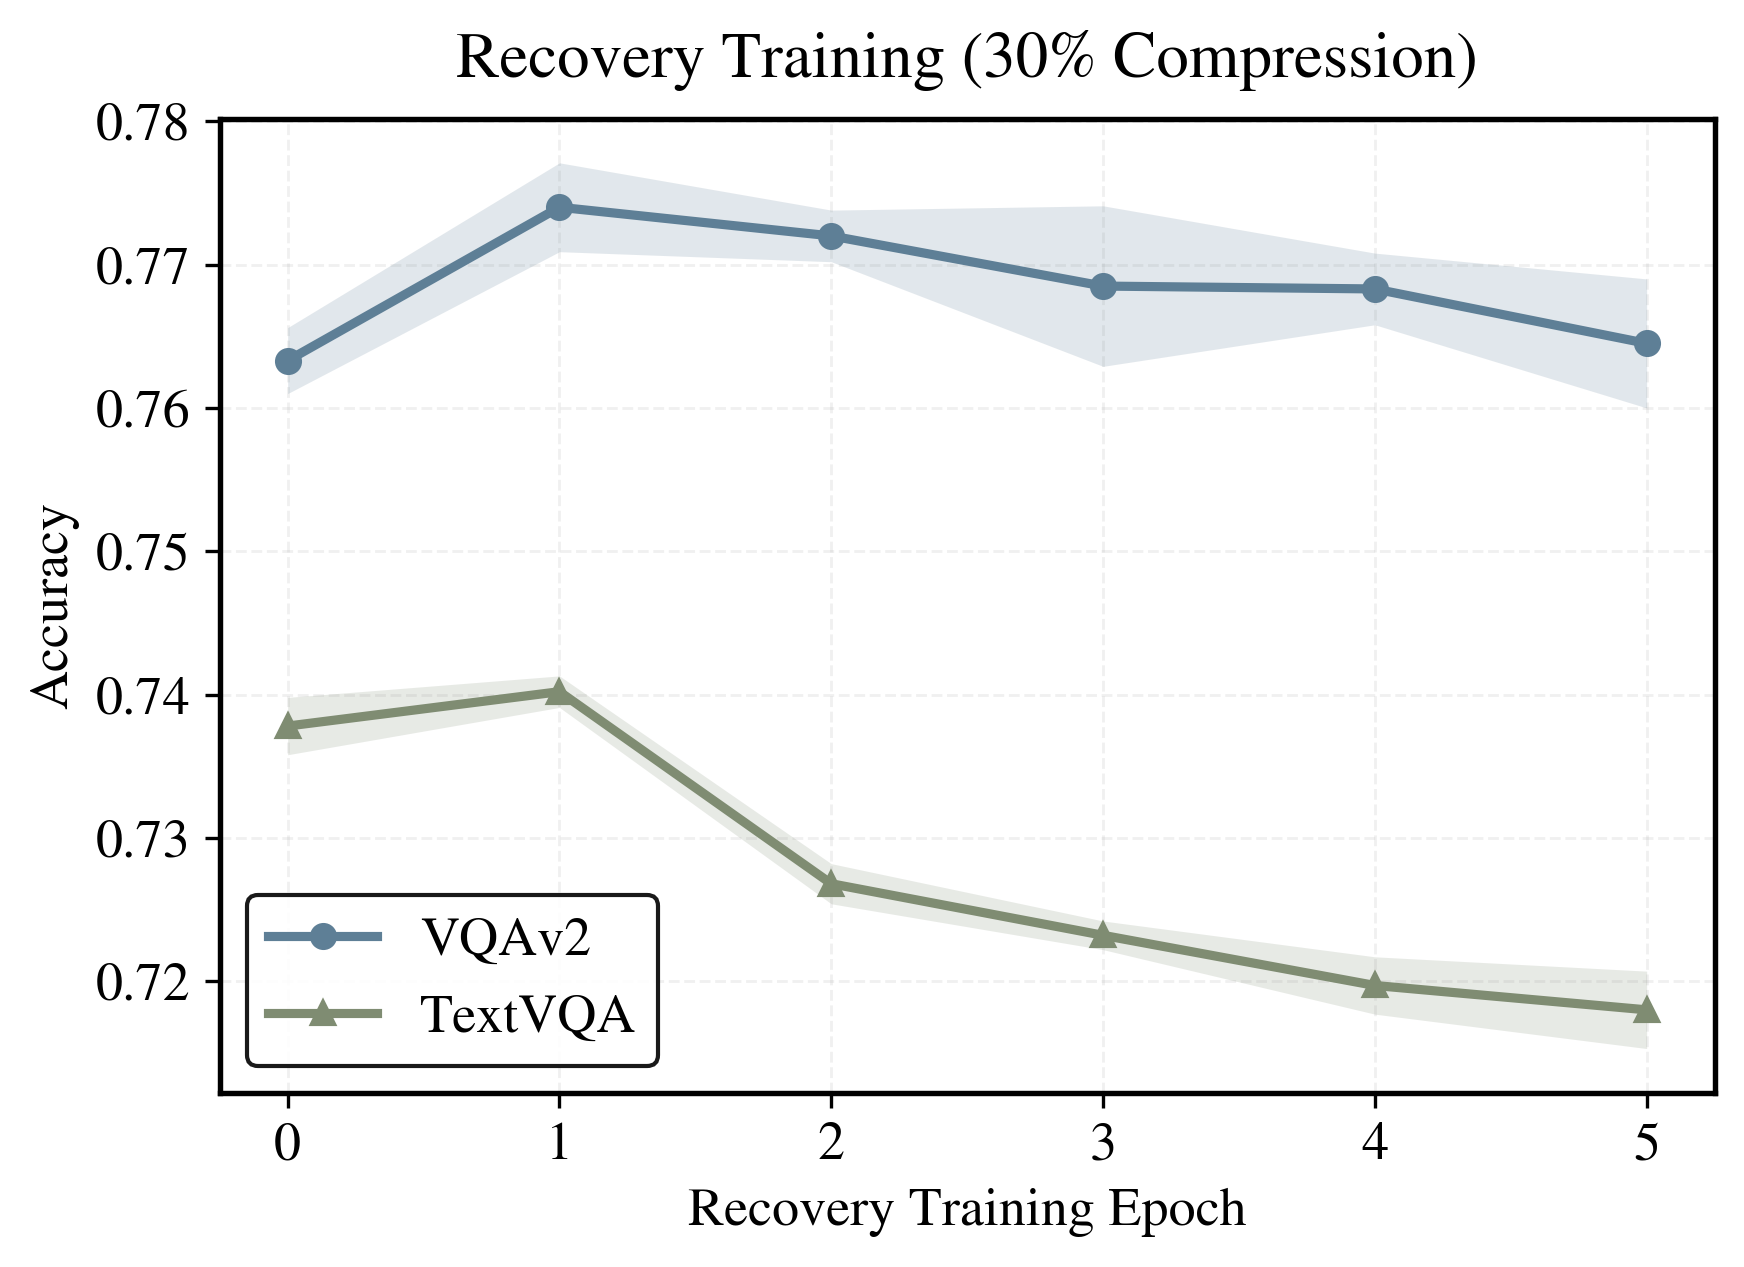
\includegraphics[width=\linewidth]{Figure/recovery.png}
    \caption{Task-specific effect of recovery training under 30\% compression.}
    % \caption{\textbf{Effect of recovery training at 30\% compression.}
    % We perform recovery training on the \textbf{target task} (VQAv2) after extracting the compressed submodel.
    % The VQAv2 accuracy increases from \textbf{0.7633} (compressed, epoch 0) to \textbf{0.7740} after one epoch,
    % while TextVQA consistently decreases (e.g., \textbf{0.7378} $\rightarrow$ \textbf{0.7180} within 5 epochs),
    % indicating that recovery training prioritizes task-specific performance rather than generalization across tasks.
    % Shaded areas denote the standard deviation.}
    \label{fig:recovery_training}
\end{figure}

\subsection{Effect of Recovery Training}

An important property of our framework is that the extracted submodel is optimized for a specific downstream task rather than preserving general-purpose capability. This design enables lightweight recovery training on the target dataset to restore task accuracy after structural compression.

We analyze this effect under a compression ratio of \textbf{30\%}, where recovery training is performed on the VQA v2 dataset. Before recovery training, the compressed model achieves an accuracy of \textbf{0.7633} on VQAv2. After one epoch of recovery training, the accuracy improves to \textbf{0.7740}, and remains relatively stable in subsequent epochs, as shown in Figure~\ref{fig:recovery_training}. These results indicate that a small amount of task-specific fine-tuning can effectively recover part of the accuracy lost during compression.

At the same time, recovery training does not improve performance on other tasks. For example, the accuracy on TextVQA decreases from \textbf{0.7378} at epoch 0 to \textbf{0.7180} after five epochs of training. This behavior reflects the task-prioritized nature of our approach: since recovery training focuses exclusively on the target dataset, the limited model capacity is gradually adapted to the target task rather than maintaining cross-task generalization.

Although the recovered VQA v2 accuracy remains lower than that of the original uncompressed model, these results demonstrate that recovery training provides an effective mechanism for restoring target-task performance after submodel extraction. This property is particularly useful in practical deployment scenarios where the model is optimized for a specific application and task-specific accuracy is more critical than preserving broad multi-task capability.


\begin{figure*}[t]
\centering
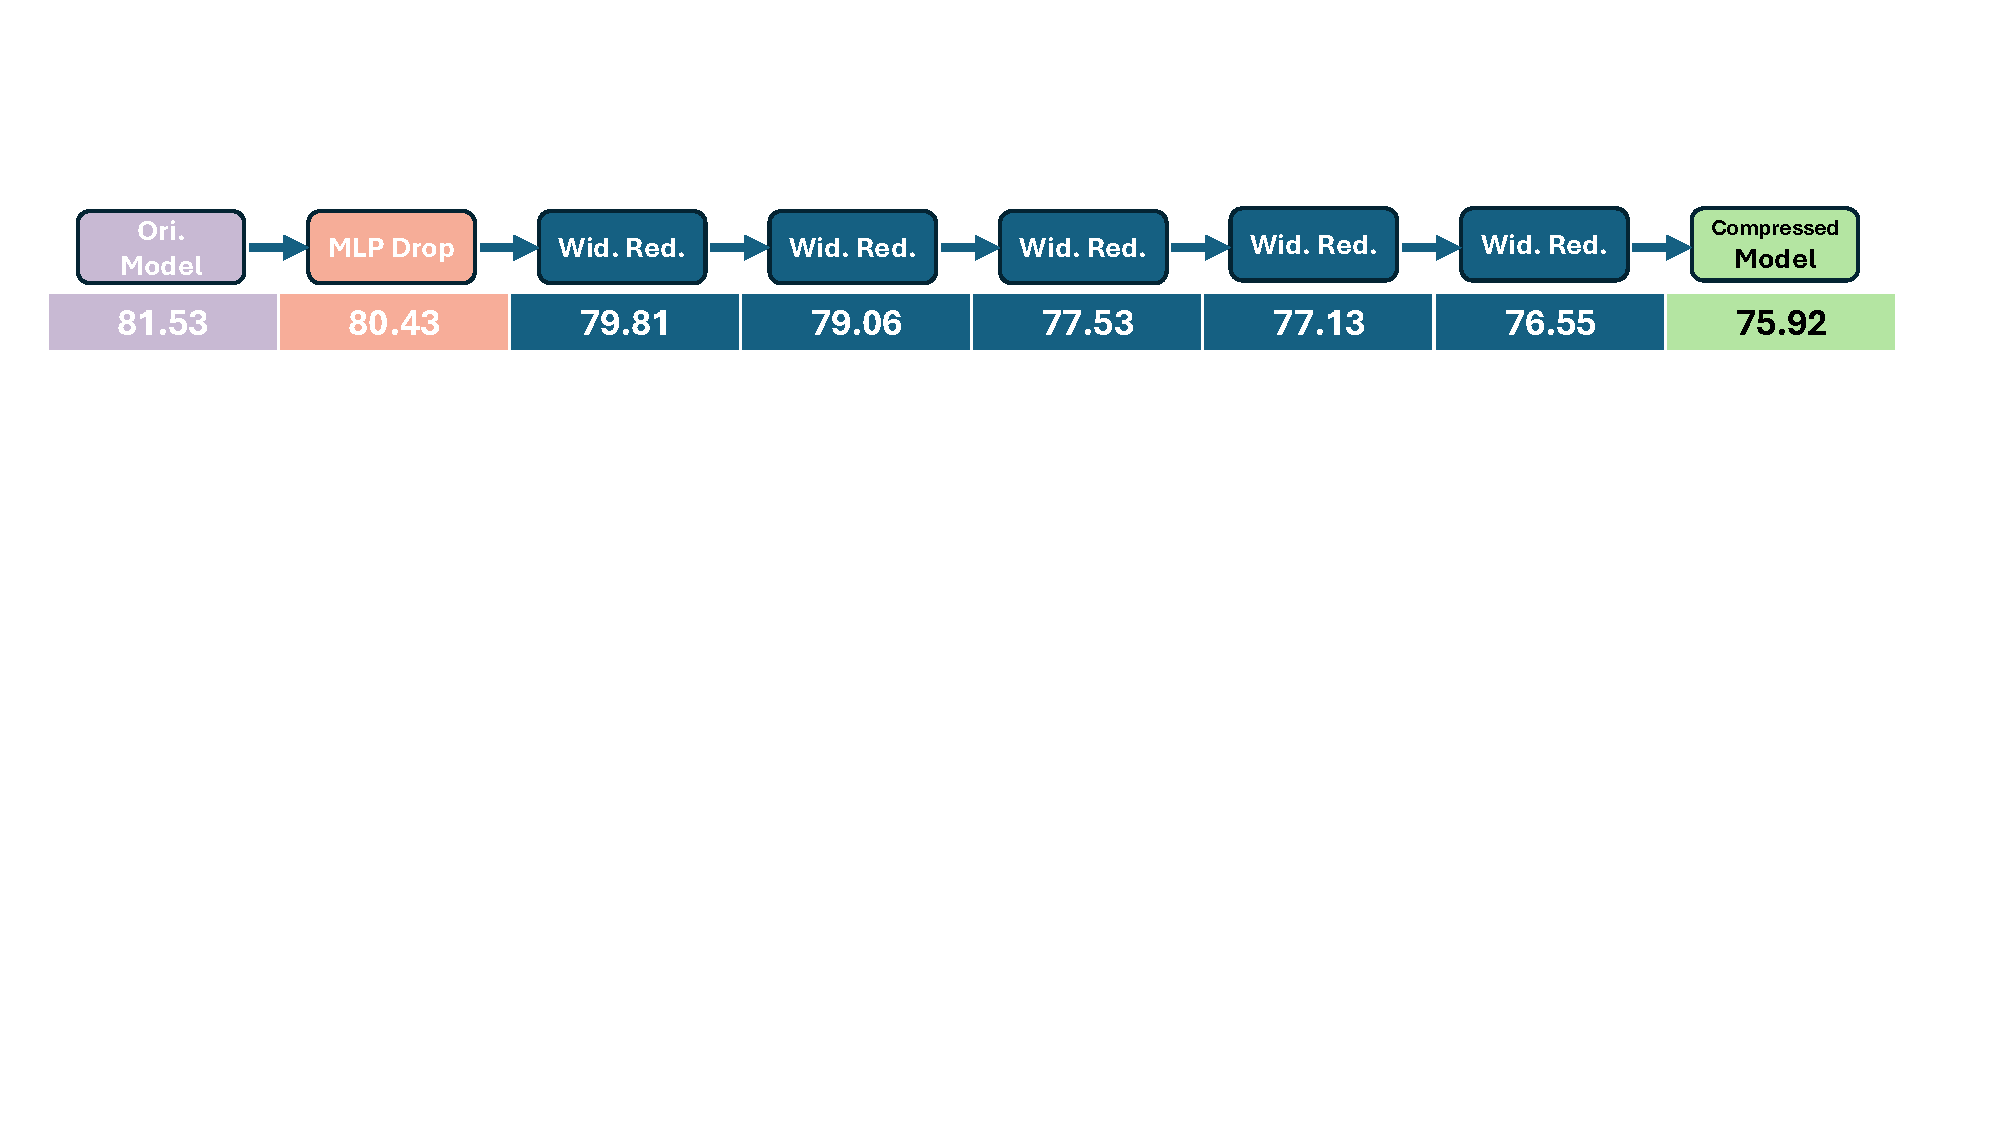
\includegraphics[width=\linewidth]{Figure/case_para.pdf}
\caption{
Greedy search trajectory under a parameter-priority constraint.
Each step shows the operator selected by the search algorithm and the corresponding model accuracy.
The search first removes MLP layers and then repeatedly applies width reduction, which provides the most favorable parameter–accuracy trade-off.
}
\label{fig:case_para}
\end{figure*}

\begin{figure*}[t]
\centering
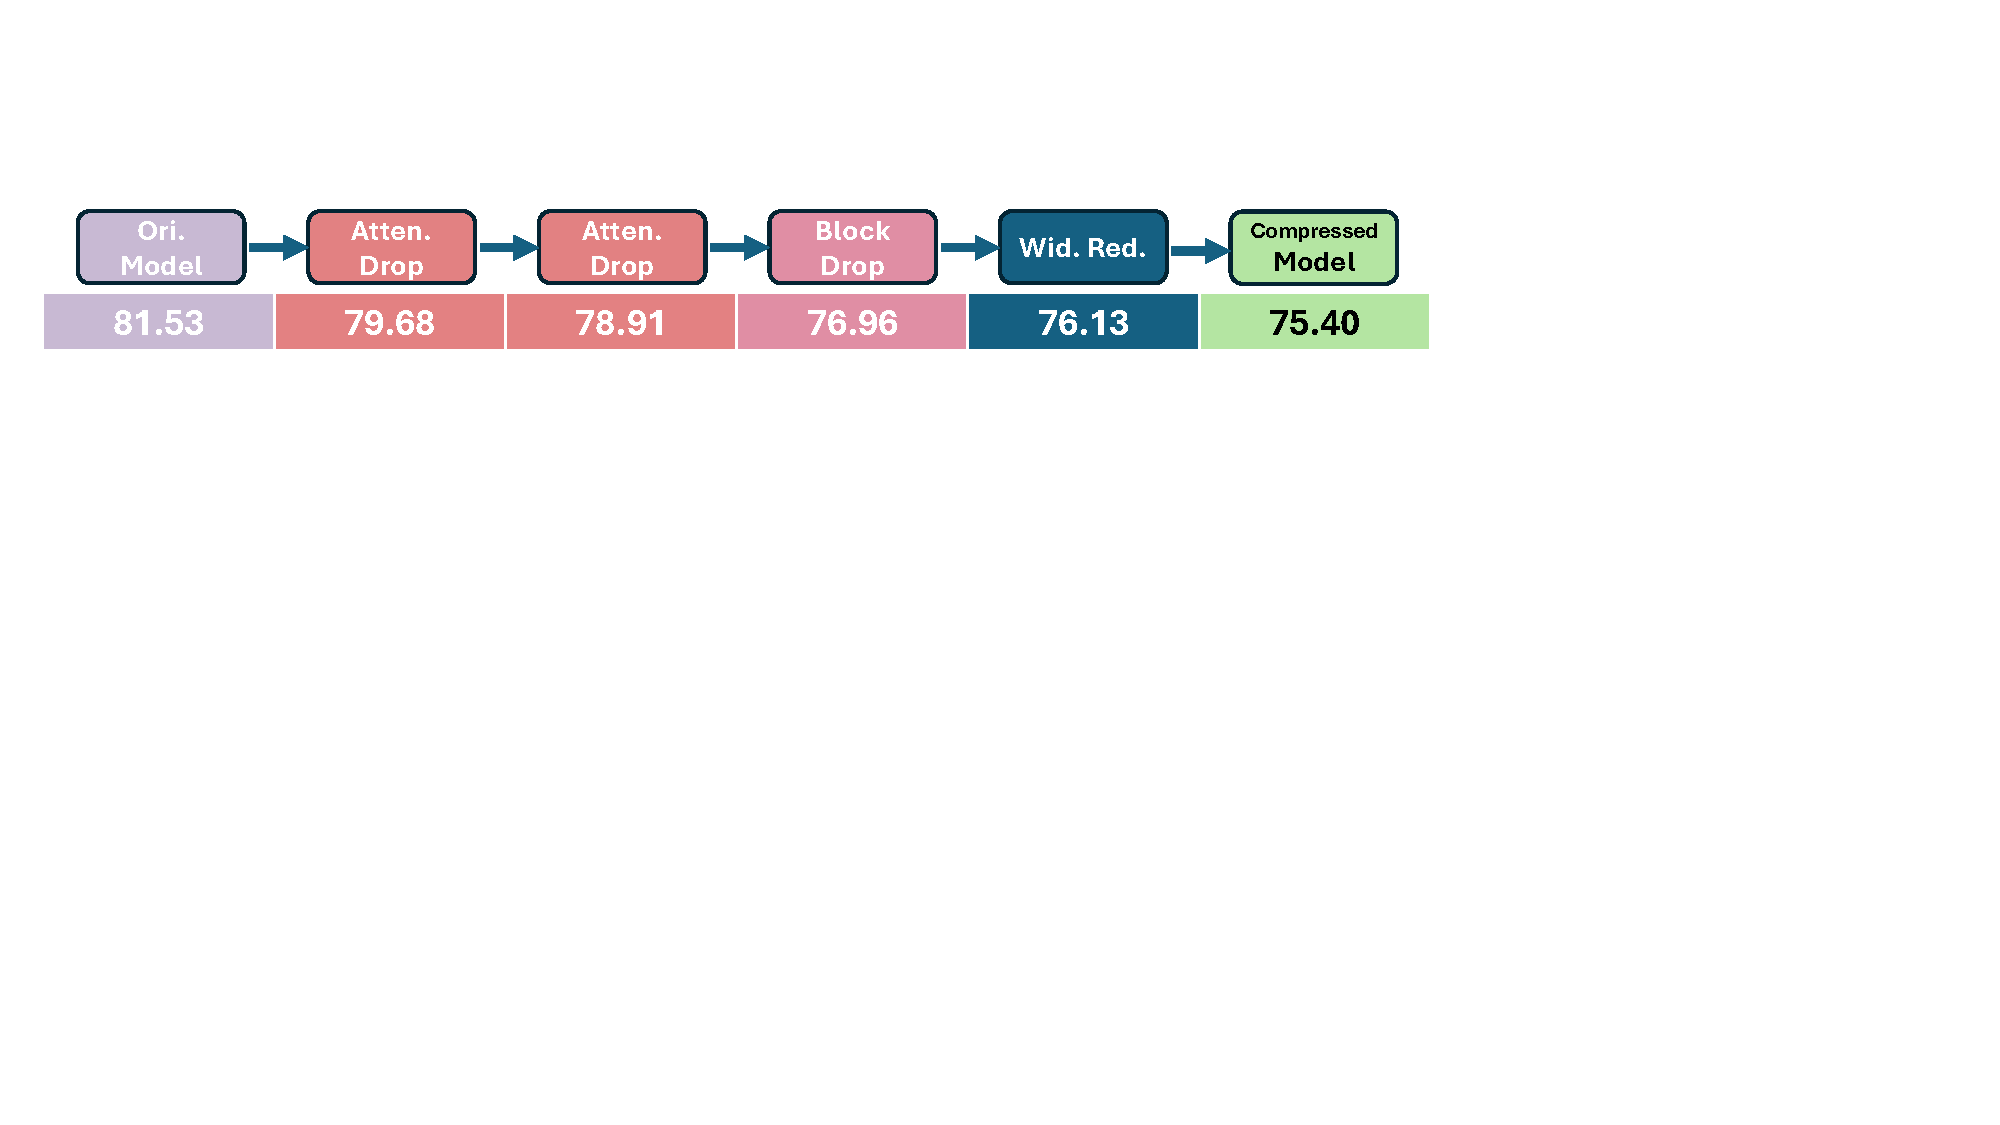
\includegraphics[width=0.8\linewidth]{Figure/case_latency.pdf}
\caption{
Greedy search trajectory under a speed-up-priority constraint.
The algorithm first removes attention layers to quickly reduce inference latency, then removes a block module, and finally applies width reduction to satisfy the remaining budget.
This demonstrates that the proposed search strategy can adaptively select different operators depending on the optimization objective.
}
\label{fig:case_latency}
\end{figure*}

\subsection{Case Study}

To better understand the behavior of the proposed submodel extraction framework, we visualize the operator selection process during the search under different deployment constraints. Figure~\ref{fig:case_para} and Figure~\ref{fig:case_latency} show two representative cases corresponding to different optimization objectives: parameter-priority and speed-up-priority.

Figure~\ref{fig:case_para} illustrates the search trajectory when parameter reduction is the primary objective. The extraction process first applies MLP Drop and then repeatedly selects width reduction in subsequent steps. This behavior reflects the strong parameter–accuracy trade-off provided by width reduction, which can effectively reduce parameter counts while preserving most of the model structure. As a result, width reduction becomes the dominant operator during the search process, gradually shrinking the model until the desired parameter budget is reached. Importantly, the accuracy degradation remains smooth throughout the process, indicating that the algorithm consistently selects operators that minimize performance loss under the parameter constraint.
In contrast, the search trajectory under the speed-up-priority setting shows a different pattern, as illustrated in Figure~\ref{fig:case_latency}. In this case, the algorithm first removes several attention layers, which directly reduces the computational cost of the model and leads to immediate inference speed improvements. After the attention layers are removed, the algorithm further applies block removal to shorten the computational path of the network. Finally, width reduction is used in the later stage to fine-tune the remaining budget and reach the desired speed-up target.

These two case studies highlight the adaptive nature of the proposed extraction framework. Instead of relying on a fixed compression strategy, the algorithm dynamically selects the most suitable operator according to the current optimization objective. Under parameter constraints it prioritizes width reduction, while under latency constraints it first removes computationally expensive modules such as attention layers. This behavior demonstrates that the proposed method can automatically discover compression strategies that align with different deployment requirements while maintaining strong task accuracy.

More broadly, the consistent search patterns observed in these cases suggest that the framework captures meaningful structural redundancy in the model. The operator selection mechanism therefore provides a practical way to adapt pretrained vision-language models to diverse deployment scenarios with different resource constraints.

% \begin{table*}[t]
% \centering
% \small
% \setlength{\tabcolsep}{2pt}
% \resizebox{\textwidth}{!}{
% \begin{tabular}{c c cc cc cc cc}
% \toprule
% \multirow{2}{*}{\textbf{Compression}} & \multirow{2}{*}{\textbf{Method}} 
% & \multicolumn{2}{c}{\textbf{QwenVL-7B}} 
% & \multicolumn{2}{c}{\textbf{QwenVL-3B}}
% & \multicolumn{2}{c}{\textbf{LLaVA-7B}}
% & \multicolumn{2}{c}{\textbf{LLaVA-13B}} \\
% \cmidrule(lr){3-4} \cmidrule(lr){5-6}
% \cmidrule(lr){7-8} \cmidrule(lr){9-10}
% & 
% & Dir. Acc & Rec. Acc 
% & Dir. Acc & Rec. Acc
% & Dir. Acc & Rec. Acc
% & Dir. Acc & Rec. Acc \\
% \midrule

% 0 & Full Model  &81.53  &  &81.83  &  &76.73  &  &79.08  &  \\
% \midrule

% \multirow{5}{*}{\textbf{5\%}} & Atten. Drop  &  &  &3.07  &39.13  &  &  &  &  \\
%      & Block Drop  &78.03  &81.73  &77.82  &78.38  &74.60  &72.07  &75.88  &76.50  \\
%      & MLP Drop  &71.13  &77.90  &79.43  &79.55  &72.88  &73.22  &74.58  &75.75  \\
%      & Width Red. &80.68  &83.82 &80.18  &80.85  &76.68  &76.22  &78.73  &79.20  \\
%      & Ours &80.68  &83.70  &80.18  &80.65  &76.68  &75.88  &  &  \\

% \midrule

% \multirow{5}{*}{\textbf{10\%}} & Atten. Drop  &  &  &  &  &  &  &  &  \\
%      & Block Drop &59.93  &70.20  &0.05  &56.33  &67.15  &63.70  &73.05  &72.03  \\
%      & MLP Drop  &70.58  &72.73  &77.48  &77.98  &70.20  &70.53  &73.60  &74.48  \\
%      & Width Red. &80.32  &82.65  &78.65  &79.05  &75.78  &75.60  &77.40  &77.12  \\
%      & Ours &80.32  &82.35  &78.65  &79.93  &75.78  &75.32  &77.43  &76.63  \\

% \midrule
% \multirow{5}{*}{\textbf{15\%}} & Atten. Drop  &  &  &  &  &  &  &  &  \\
%      & Block Drop   &6.87  &52.25  &0.05  &12.03  &63.55  &61.78  &22.13  &57.97  \\
%      & MLP Drop  &19.57  &57.87  &51.07  &73.17  &65.88  &66.85  &69.28  &71.15  \\
%      & Width Red. &80.45  &81.78  &77.53  &77.92  &74.48  &74.27  &76.77  &76.65  \\
%      & Ours &80.45  &81.80  &77.53  &77.95  &74.48  &74.23  &75.43  &75.33  \\
     
% \midrule
% \multirow{5}{*}{\textbf{20\%}} & Atten. Drop  &  &  &  &  &  &  &  &  \\
%      & Block Drop  &4.83  &23.88  &0.10  &0.40  &52.83  &47.92  &17.32  &46.80  \\
%      & MLP Drop  &0.00  &7.97  &14.60  &62.03  &53.62  &54.13  &64.43  &67.07  \\
%      & Width Red. &79.77  &81.07  &75.92 &77.05  &71.63  &70.25  &75.47  &75.42  \\
%      & Ours &79.77  &80.97  &75.92  &76.95  &71.63  &70.35  &74.53  &73.97  \\

% \midrule
% \multirow{5}{*}{\textbf{25\%}} & Atten. Drop  &  &  &  &  &  &  &  &  \\
%      & Block Drop  &0.63  &9.05  &0.10  &0.42  &45.87  &43.82  &11.02  &49.82  \\
%      & MLP Drop  &0.00  &0.65  &2.95  &44.15  &31.40  &42.62  &56.08  &56.92  \\
%      & Width Red. &77.98  &79.15  &73.73  &74.45  &65.30  &63.03  &73.18  &73.43  \\
%      & Ours &77.98  &79.03  &73.73  &74.13  &65.30  &63.07  &71.53  &71.33  \\

% \midrule
% \multirow{5}{*}{\textbf{30\%}} & Atten. Drop  &  &  &  &  &  &  &  &  \\
%      & Block Drop   &0.32  &4.92  &0.05  &0.48  &35.57  &39.27  &14.17  &45.10  \\
%      & MLP Drop        &0.00  &0.17  &0.20  &1.95  &10.60  &37.53  &37.90  &38.12  \\
%      & Width Red. &76.33 &77.35 &69.52  &70.77  &57.03  &54.40  &69.02  &68.50  \\
%      & Ours &76.33  &77.28  &69.52  &70.30  &57.03  &54.37  &66.98  &68.87  \\

% % \midrule
% % \multirow{5}{*}{\textbf{40\%}} & Atten. Drop  &  &  &  &  &  &  &  &  \\
% %      & Block Drop      &  &  &  &  &  &  &  &  \\
% %      & MLP Drop        &  &  &  &  &  &  &  &  \\
% %      & Width Red. &  &  &  &  &  &  &  &  \\
% %      & Ours &  &  &  &  &  &  &  &  \\

% % \midrule
% % \multirow{5}{*}{\textbf{50\%}} & Atten. Drop  &  &  &  &  &  &  &  &  \\
% %      & Block Drop      &  &  &  &  &  &  &  &  \\
% %      & MLP Drop        &  &  &  &  &  &  &  &  \\
% %      & Width Red. &  &  &  &  &  &  &  &  \\
% %      & Ours &  &  &  &  &  &  &  &  \\

% \bottomrule
% \end{tabular}
% }
% \caption{Comparison of different compression strategies under varying compression ratios. 
% Direct Acc denotes performance immediately after structural reduction. 
% Recovery Acc denotes performance after lightweight task-specific recovery. \textbf{VQAV2}}
% \label{tab:compression_results1}
% \end{table*}



% \begin{table}[t]
% \centering
% \caption{Inference Speed Comparison (VQAv2 Val).}
% \label{tab:speed_random_drop}
% \begin{tabular}{l c c c}
% \toprule
% Method & Drop Ratio & Tokens/sec & Speedup ($\times$) \\
% \midrule
% Baseline & --  & 24.68 & 1.00 \\
% \midrule
% MLP Drop        & 0.1 & 24.60 &0.9912 \\
% Block Drop      & 0.1 & 24.67 &0.9941  \\
% Width Reduction & 0.1 & 26.61 & 1.0724 \\
% \midrule
% MLP Drop        & 0.2 & 43.35 &1.7564 \\
% Block Drop      & 0.2 & 35.73 &1.4478  \\
% Width Reduction & 0.2 & 28.76 & 1.1653 \\
% \midrule
% MLP Drop        & 0.3 & 88.58 & 3.5264 \\
% Block Drop      & 0.3 & 32.82 & 1.3067 \\
% Width Reduction & 0.3 & 83.42 & 3.3211\\
% \midrule
% MLP Drop        & 0.4 & 92.02 & 3.6045 \\
% Block Drop      & 0.4 & 90.31 & 3.5374 \\
% Width Reduction & 0.4 & 92.98 & 3.6418\\
% \midrule
% MLP Drop        & 0.5 & 88.43 &3.5759 \\
% Block Drop      & 0.5 & 91.66 &3.7065 \\
% Width Reduction & 0.5 & 79.97 &3.2336 \\
% \bottomrule
% \end{tabular}
% \end{table}

\section{Conclusion}

In this work, we revisit model compression from a deployment-oriented perspective and formulate \emph{budget-aware, task-conditioned submodel extraction} for VLMs. Rather than preserving universal zero-shot capability, we focus on practical deployment settings where models operate on a small number of target tasks under explicit computational constraints. Through systematic analysis of representative structural compression strategies, including attention drop, MLP drop, block drop, and MLP width reduction, we observe distinct trade-offs among efficiency, parameter reduction, and task performance. In particular, width reduction consistently preserves task performance better under comparable budgets, suggesting that redundancy in many VLMs is more concentrated in MLP width than model depth. Motivated by these findings, we propose a unified framework that automatically extracts task-specific submodels under a given parameter budget by combining model-level importance ranking with granularity-aware extraction. Extensive experiments on multiple Qwen-based and LLaVA-based VLMs demonstrate that our method consistently maintains strong task accuracy under substantial parameter reduction. Overall, our work provides a practical and scalable pathway for transforming large pretrained foundation models into task-aligned and budget-efficient models for real-world deployment.

% \section{Conclusion}

% In this work, we revisit model compression from a deployment-oriented perspective and formulate \emph{budget-aware, task-conditioned submodel extraction} for VLMs. Instead of preserving universal zero-shot capability, we emphasize that practical deployment scenarios typically involve a small number of target tasks operating under explicit computational constraints. From this perspective, extracting task-aligned submodels becomes essential for bridging the gap between large-scale pretraining and real-world deployment. Through systematic analysis of representative structural compression strategies in transformer-based vision-language models, including attention drop, MLP drop, block drop, and MLP width reduction, we observe clear differences in their behavior. Attention drop mainly improves inference efficiency with minimal parameter reduction, while block drop provides large parameter savings but often leads to significant performance degradation due to its coarse granularity. MLP drop offers moderate compression but becomes unstable at higher reduction ratios, whereas width reduction consistently preserves task performance better under comparable budgets, suggesting that redundancy in many VLMs is more concentrated in MLP width than in model depth.

% Building on these observations, we propose a unified framework that automatically extracts task-specific submodels under a given parameter budget. By combining model-level importance ranking with a granularity-controlled extraction process, the proposed method adaptively selects among heterogeneous structural reductions and dynamically determines the most effective compression strategy at each reduction step. This design enables the framework to flexibly construct high-performing submodels across a wide range of compression ratios without modifying the original pretraining process. Extensive experiments on multiple Qwen-based and LLaVA-based vision-language models demonstrate that our method consistently achieves strong task accuracy under significant parameter reductions. More broadly, our work provides a practical and scalable pathway for transforming large pretrained foundation models into task-aligned and budget-efficient models suitable for real-world deployment.

\section*{Limitations}

Our framework focuses on task-conditioned submodel extraction under specific deployment constraints, and therefore primarily evaluates performance on a small set of VQA-style benchmarks and representative VLM architectures. Although the proposed extraction strategy generalizes across multiple compression operators, additional studies on broader multimodal tasks, larger-scale models, and more diverse deployment scenarios would further improve the understanding of its applicability. In addition, the current framework relies on lightweight validation-based ranking and greedy operator selection, which provides strong empirical performance while not guaranteeing globally optimal submodel configurations under a given budget.

% \section*{Acknowledgments}

% This document has been adapted
% by Steven Bethard, Ryan Cotterell and Rui Yan
% from the instructions for earlier ACL and NAACL proceedings, including those for
% ACL 2019 by Douwe Kiela and Ivan Vuli\'{c},
% NAACL 2019 by Stephanie Lukin and Alla Roskovskaya,
% ACL 2018 by Shay Cohen, Kevin Gimpel, and Wei Lu,
% NAACL 2018 by Margaret Mitchell and Stephanie Lukin,
% Bib\TeX{} suggestions for (NA)ACL 2017/2018 from Jason Eisner,
% ACL 2017 by Dan Gildea and Min-Yen Kan,
% NAACL 2017 by Margaret Mitchell,
% ACL 2012 by Maggie Li and Michael White,
% ACL 2010 by Jing-Shin Chang and Philipp Koehn,
% ACL 2008 by Johanna D. Moore, Simone Teufel, James Allan, and Sadaoki Furui,
% ACL 2005 by Hwee Tou Ng and Kemal Oflazer,
% ACL 2002 by Eugene Charniak and Dekang Lin,
% and earlier ACL and EACL formats written by several people, including
% John Chen, Henry S. Thompson and Donald Walker.
% Additional elements were taken from the formatting instructions of the \emph{International Joint Conference on Artificial Intelligence} and the \emph{Conference on Computer Vision and Pattern Recognition}.

% Bibliography entries for the entire Anthology, followed by custom entries
%\bibliography{custom,anthology-overleaf-1,anthology-overleaf-2}

% Custom bibliography entries only
\bibliography{custom}

\appendix

% \section{Example Appendix}
% \label{sec:appendix}

% This is an appendix.

\end{document}
